\documentclass[twoside]{book}

% Packages required by doxygen
\usepackage{fixltx2e}
\usepackage{calc}
\usepackage{doxygen}
\usepackage[export]{adjustbox} % also loads graphicx
\usepackage{graphicx}
\usepackage[utf8]{inputenc}
\usepackage{makeidx}
\usepackage{multicol}
\usepackage{multirow}
\PassOptionsToPackage{warn}{textcomp}
\usepackage{textcomp}
\usepackage[nointegrals]{wasysym}
\usepackage[table]{xcolor}

% Font selection
\usepackage[T1]{fontenc}
\usepackage[scaled=.90]{helvet}
\usepackage{courier}
\usepackage{amssymb}
\usepackage{sectsty}
\renewcommand{\familydefault}{\sfdefault}
\allsectionsfont{%
  \fontseries{bc}\selectfont%
  \color{darkgray}%
}
\renewcommand{\DoxyLabelFont}{%
  \fontseries{bc}\selectfont%
  \color{darkgray}%
}
\newcommand{\+}{\discretionary{\mbox{\scriptsize$\hookleftarrow$}}{}{}}

% Page & text layout
\usepackage{geometry}
\geometry{%
  a4paper,%
  top=2.5cm,%
  bottom=2.5cm,%
  left=2.5cm,%
  right=2.5cm%
}
\tolerance=750
\hfuzz=15pt
\hbadness=750
\setlength{\emergencystretch}{15pt}
\setlength{\parindent}{0cm}
\setlength{\parskip}{3ex plus 2ex minus 2ex}
\makeatletter
\renewcommand{\paragraph}{%
  \@startsection{paragraph}{4}{0ex}{-1.0ex}{1.0ex}{%
    \normalfont\normalsize\bfseries\SS@parafont%
  }%
}
\renewcommand{\subparagraph}{%
  \@startsection{subparagraph}{5}{0ex}{-1.0ex}{1.0ex}{%
    \normalfont\normalsize\bfseries\SS@subparafont%
  }%
}
\makeatother

% Headers & footers
\usepackage{fancyhdr}
\pagestyle{fancyplain}
\fancyhead[LE]{\fancyplain{}{\bfseries\thepage}}
\fancyhead[CE]{\fancyplain{}{}}
\fancyhead[RE]{\fancyplain{}{\bfseries\leftmark}}
\fancyhead[LO]{\fancyplain{}{\bfseries\rightmark}}
\fancyhead[CO]{\fancyplain{}{}}
\fancyhead[RO]{\fancyplain{}{\bfseries\thepage}}
\fancyfoot[LE]{\fancyplain{}{}}
\fancyfoot[CE]{\fancyplain{}{}}
\fancyfoot[RE]{\fancyplain{}{\bfseries\scriptsize Generated by Doxygen }}
\fancyfoot[LO]{\fancyplain{}{\bfseries\scriptsize Generated by Doxygen }}
\fancyfoot[CO]{\fancyplain{}{}}
\fancyfoot[RO]{\fancyplain{}{}}
\renewcommand{\footrulewidth}{0.4pt}
\renewcommand{\chaptermark}[1]{%
  \markboth{#1}{}%
}
\renewcommand{\sectionmark}[1]{%
  \markright{\thesection\ #1}%
}

% Indices & bibliography
\usepackage{natbib}
\usepackage[titles]{tocloft}
\setcounter{tocdepth}{3}
\setcounter{secnumdepth}{5}
\makeindex

% Hyperlinks (required, but should be loaded last)
\usepackage{ifpdf}
\ifpdf
  \usepackage[pdftex,pagebackref=true]{hyperref}
\else
  \usepackage[ps2pdf,pagebackref=true]{hyperref}
\fi
\hypersetup{%
  colorlinks=true,%
  linkcolor=blue,%
  citecolor=blue,%
  unicode%
}

% Custom commands
\newcommand{\clearemptydoublepage}{%
  \newpage{\pagestyle{empty}\cleardoublepage}%
}

\usepackage{caption}
\captionsetup{labelsep=space,justification=centering,font={bf},singlelinecheck=off,skip=4pt,position=top}

%===== C O N T E N T S =====

\begin{document}

% Titlepage & ToC
\hypersetup{pageanchor=false,
             bookmarksnumbered=true,
             pdfencoding=unicode
            }
\pagenumbering{roman}
\begin{titlepage}
\vspace*{7cm}
\begin{center}%
{\Large Dy\+Ba O\+RF }\\
\vspace*{1cm}
{\large Generated by Doxygen 1.8.11}\\
\end{center}
\end{titlepage}
\clearemptydoublepage
\tableofcontents
\clearemptydoublepage
\pagenumbering{arabic}
\hypersetup{pageanchor=true}

%--- Begin generated contents ---
\chapter{R\+E\+A\+D\+ME}
\label{md__Users_guotaiwang_Documents_workspace_git_repository_DyBaORF_README}
\hypertarget{md__Users_guotaiwang_Documents_workspace_git_repository_DyBaORF_README}{}
Dy\+Ba O\+RF \begin{DoxyVerb}DyBa ORF is a Dymanically Balanced Online Random Forest, which addresses three problems in learning with Random Forests: 

1). Online learning. It can accept gradually arrived training data and update the model on-the-fly.
2). Data imbalance. It deals with imbalanced data of different classes, avoiding low correct rate of classification for minor class.
3). Changing imbalance ratio. The ratio (degree) of imbalance may dynamically change when new training data arrive sequentially. Compared with traditionaly Online Random Forest (Saffari, A. 2009, Barinova, O. 2012) which assumes the imblance ratio do not change,
DyBa ORF updates the model dynamically with the ability to be adapted to new imbalance ratio.
\end{DoxyVerb}


Author Info \begin{DoxyVerb}DyBa ORF was developed as part of the GIFT-Surg project. The algorithm and software were developed by Guotai Wang at the Translational Imaging Group in the Centre for Medical Image Computing at University College London (UCL).

If you use this software, please cite this paper:
Guotai Wang, Maria A. Zuluaga, Rosalind Pratt, Michael Aertsen, Tom Doel, Maria Klusmann, Anna L. David, Jan Deprest, Tom Vercauteren, Sebastien Ourselin
Dynamically Balanced Online Random Forests for Interactive Segmentation, MICCAI 2016. (accepted)
\end{DoxyVerb}


Software links \begin{DoxyVerb}Slic-Seg home page: http://www.gift-surg.ac.uk/
Translational Imaging Group: http://cmictig.cs.ucl.ac.uk/
GitHub mirror.
\end{DoxyVerb}


License \begin{DoxyVerb}Copyright (c) 2014-2016, University College London.

DyBa ORF is available as free open-source software under a BSD 3-Clause License. Other licenses may apply for dependencies:
\end{DoxyVerb}


System requirements \begin{DoxyVerb}The current version of DyBa ORF requries:

A C++ compiler installed and configured to work with cmake.
Cmake to generate the project from source code.
\end{DoxyVerb}


How to use \begin{DoxyVerb}Suppose the source code directory is $DyBaORF.
Switch to the $DyBaORF directory.
Open Cmake, set the source code directory as $DyBaORF, and set the build directory as $DyBaORF/build.
Click Configure, select the c++ compile you use. (VS in Windows, Clang++ in Mac, gcc in Linux)
Click Generate to generate the project, which can be found at $DyBaORF/build.
Go to $DyBaORF/build to open the generated project, compile it and then you can run it.
\end{DoxyVerb}


Funding \begin{DoxyVerb}This work was supported through an Innovative Engineering for Health award by the Wellcome Trust [WT101957], the Engineering and Physical Sciences Research Council (EPSRC) [NS/A000027/1] and a National Institute for Health Research Biomedical Research Centre UCLH/UCL High Impact Initiative, A UCL Overseas Research Scholarship and a UCL Graduate Research Scholarship.
\end{DoxyVerb}


Supported Platforms \begin{DoxyVerb}DyBa ORF is a cross-platform C++ library. It supports Windows, Mac and Linux.\end{DoxyVerb}
 
\chapter{Hierarchical Index}
\section{Class Hierarchy}
This inheritance list is sorted roughly, but not completely, alphabetically\+:\begin{DoxyCompactList}
\item \contentsline{section}{Abstract\+Test\+Example}{\pageref{class_abstract_test_example}}{}
\begin{DoxyCompactList}
\item \contentsline{section}{R\+F\+Test\+Example}{\pageref{class_r_f_test_example}}{}
\end{DoxyCompactList}
\item \contentsline{section}{Random\+Forest\+:\+:Node$<$ T $>$}{\pageref{class_random_forest_1_1_node}}{}
\item \contentsline{section}{Random\+Forest\+:\+:O\+D\+Tree$<$ T $>$}{\pageref{class_random_forest_1_1_o_d_tree}}{}
\item \contentsline{section}{Random\+Forest\+:\+:O\+R\+Forest$<$ T $>$}{\pageref{class_random_forest_1_1_o_r_forest}}{}
\end{DoxyCompactList}

\chapter{Class Index}
\section{Class List}
Here are the classes, structs, unions and interfaces with brief descriptions\+:\begin{DoxyCompactList}
\item\contentsline{section}{\hyperlink{class_abstract_test_example}{Abstract\+Test\+Example} \\*Class \hyperlink{class_abstract_test_example}{Abstract\+Test\+Example} }{\pageref{class_abstract_test_example}}{}
\item\contentsline{section}{\hyperlink{class_random_forest_1_1_node}{Random\+Forest\+::\+Node$<$ T $>$} \\*Class \hyperlink{class_random_forest_1_1_node}{Node} }{\pageref{class_random_forest_1_1_node}}{}
\item\contentsline{section}{\hyperlink{class_random_forest_1_1_o_d_tree}{Random\+Forest\+::\+O\+D\+Tree$<$ T $>$} \\*Class \hyperlink{class_random_forest_1_1_o_d_tree}{O\+D\+Tree} }{\pageref{class_random_forest_1_1_o_d_tree}}{}
\item\contentsline{section}{\hyperlink{class_random_forest_1_1_o_r_forest}{Random\+Forest\+::\+O\+R\+Forest$<$ T $>$} \\*Class \hyperlink{class_random_forest_1_1_o_r_forest}{O\+R\+Forest} }{\pageref{class_random_forest_1_1_o_r_forest}}{}
\item\contentsline{section}{\hyperlink{class_r_f_test_example}{R\+F\+Test\+Example} \\*Class \hyperlink{class_r_f_test_example}{R\+F\+Test\+Example} }{\pageref{class_r_f_test_example}}{}
\end{DoxyCompactList}

\chapter{Class Documentation}
\hypertarget{class_abstract_test_example}{}\section{Abstract\+Test\+Example Class Reference}
\label{class_abstract_test_example}\index{Abstract\+Test\+Example@{Abstract\+Test\+Example}}


class \hyperlink{class_abstract_test_example}{Abstract\+Test\+Example}  




{\ttfamily \#include $<$Abstract\+Test\+Example.\+h$>$}

Inheritance diagram for Abstract\+Test\+Example\+:\begin{figure}[H]
\begin{center}
\leavevmode
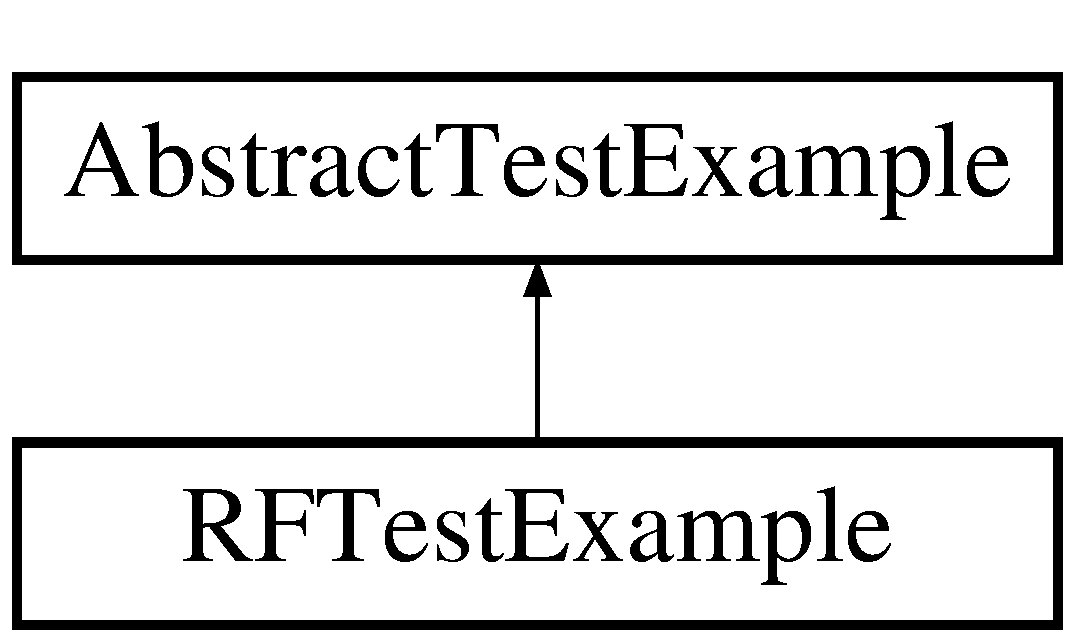
\includegraphics[height=2.000000cm]{class_abstract_test_example}
\end{center}
\end{figure}
\subsection*{Public Member Functions}
\begin{DoxyCompactItemize}
\item 
\hyperlink{class_abstract_test_example_aba49e3392989d9bd96f01a570c0b1136}{Abstract\+Test\+Example} ()
\item 
\hyperlink{class_abstract_test_example_aea4e826ad11ebf45f1ec9a70eacd60eb}{$\sim$\+Abstract\+Test\+Example} ()
\item 
bool \hyperlink{class_abstract_test_example_a61d97ab0e5ff9496902168c09ac733e9}{Load\+Data} (Data\+Set\+Name data)
\item 
void \hyperlink{class_abstract_test_example_af0c5621acae6f8b30f372517a7dacbe5}{Set\+Train\+Data\+Chunk} (double start\+Percent, double end\+Percent, double increase\+Percent)
\item 
virtual void \hyperlink{class_abstract_test_example_a7ad10a9fa18201ab05fc27528a8b52e6}{Run} (int Max\+Iter)
\item 
virtual void \hyperlink{class_abstract_test_example_ab887dba326820db0a9c896ec83559e75}{Print\+Performance} ()
\item 
void \hyperlink{class_abstract_test_example_a785757c20c8467927495481b56d12e67}{Print\+Data\+Information} ()
\end{DoxyCompactItemize}
\subsection*{Protected Member Functions}
\begin{DoxyCompactItemize}
\item 
bool \hyperlink{class_abstract_test_example_acbe2d5227fbf31c3e768d76cd2d49790}{Load\+C\+T\+G\+Data\+Set} ()
\item 
bool \hyperlink{class_abstract_test_example_a29817803c059137758d418b0d4121cd9}{Load\+Wine\+Data\+Set} ()
\item 
bool \hyperlink{class_abstract_test_example_a634004a9e97c8dc30ad14a38f670533e}{Load\+Musk\+Data\+Set} ()
\item 
bool \hyperlink{class_abstract_test_example_aeadf20fc41aaef160c6c054e8c2fb78e}{Load\+Biodeg\+Data\+Set} ()
\item 
void \hyperlink{class_abstract_test_example_ac54e0a9bf455ff3dc3a18d919b13c667}{Update\+Data\+Info} ()
\item 
void \hyperlink{class_abstract_test_example_a384c5ea404dd331a15713049175e56d6}{Generate\+Train\+And\+Test\+Data} ()
\item 
void \hyperlink{class_abstract_test_example_a18d6eb7fa348dc8b1615411d6094b43e}{Set\+Train\+Data\+Online} (int start\+Index, int end\+Index)
\item 
std\+::vector$<$ double $>$ \hyperlink{class_abstract_test_example_a70819a22ccef5619db2bbbd51088701d}{Get\+Imbalance\+Ratio} ()
\item 
int \hyperlink{class_abstract_test_example_ab3caa48f410285ef782896388aa57cef}{Get\+TrainN} () const 
\item 
void \hyperlink{class_abstract_test_example_acae6617be7fdb7c16284c132c850d139}{Get\+Mean\+And\+Std} (std\+::vector$<$ std\+::vector$<$ double $>$ $>$ i\+\_\+array, std\+::vector$<$ double $>$ $\ast$o\+\_\+mean, std\+::vector$<$ double $>$ $\ast$o\+\_\+std)
\end{DoxyCompactItemize}
\subsection*{Protected Attributes}
\begin{DoxyCompactItemize}
\item 
int {\bfseries featureN}\hypertarget{class_abstract_test_example_a8796ab8a714c67f838a10c10c7ddde41}{}\label{class_abstract_test_example_a8796ab8a714c67f838a10c10c7ddde41}

\item 
int {\bfseries instanceN}\hypertarget{class_abstract_test_example_a55a605c68cdbc8b406d5e6ecdaac5a92}{}\label{class_abstract_test_example_a55a605c68cdbc8b406d5e6ecdaac5a92}

\item 
int {\bfseries positiveN}\hypertarget{class_abstract_test_example_a584a810365ae5dccc6557b3bd1ccdd7f}{}\label{class_abstract_test_example_a584a810365ae5dccc6557b3bd1ccdd7f}

\item 
int {\bfseries negtiveN}\hypertarget{class_abstract_test_example_acb3cf119e5d6b8a905a174dd09983bb5}{}\label{class_abstract_test_example_acb3cf119e5d6b8a905a174dd09983bb5}

\item 
int {\bfseries trainN}\hypertarget{class_abstract_test_example_a2b9f6b567af1cc6d330d9a559d9f56e7}{}\label{class_abstract_test_example_a2b9f6b567af1cc6d330d9a559d9f56e7}

\item 
int {\bfseries testN}\hypertarget{class_abstract_test_example_a88ee381aa7edca9bc06d8047515bf78c}{}\label{class_abstract_test_example_a88ee381aa7edca9bc06d8047515bf78c}

\item 
int {\bfseries pos\+Ntrain}\hypertarget{class_abstract_test_example_a672e3add0ce9d409ca9f71dc7da77979}{}\label{class_abstract_test_example_a672e3add0ce9d409ca9f71dc7da77979}

\item 
int {\bfseries neg\+Ntrain}\hypertarget{class_abstract_test_example_acc333780fd867a9ade3177841a17cae6}{}\label{class_abstract_test_example_acc333780fd867a9ade3177841a17cae6}

\item 
int {\bfseries pos\+Ntest}\hypertarget{class_abstract_test_example_a1c42b89539ddae8b3605e25bb298b015}{}\label{class_abstract_test_example_a1c42b89539ddae8b3605e25bb298b015}

\item 
int {\bfseries neg\+Ntest}\hypertarget{class_abstract_test_example_a8cab291349e5da4b03eee463156916d5}{}\label{class_abstract_test_example_a8cab291349e5da4b03eee463156916d5}

\item 
std\+::shared\+\_\+ptr$<$ std\+::vector$<$ std\+::shared\+\_\+ptr$<$ std\+::vector$<$ double $>$ $>$ $>$ $>$ {\bfseries origin\+Data}\hypertarget{class_abstract_test_example_a8f79d0ca14dcd405089698c9223ede30}{}\label{class_abstract_test_example_a8f79d0ca14dcd405089698c9223ede30}

\item 
std\+::shared\+\_\+ptr$<$ std\+::vector$<$ std\+::shared\+\_\+ptr$<$ std\+::vector$<$ double $>$ $>$ $>$ $>$ {\bfseries train\+Data}\hypertarget{class_abstract_test_example_ae2565b00a6090a55b5bce07246a33f56}{}\label{class_abstract_test_example_ae2565b00a6090a55b5bce07246a33f56}

\item 
std\+::shared\+\_\+ptr$<$ std\+::vector$<$ std\+::shared\+\_\+ptr$<$ std\+::vector$<$ double $>$ $>$ $>$ $>$ {\bfseries test\+Data}\hypertarget{class_abstract_test_example_aa44ef857d822f6c13174ebf4023ca765}{}\label{class_abstract_test_example_aa44ef857d822f6c13174ebf4023ca765}

\item 
std\+::vector$<$ int $>$ {\bfseries train\+Index\+Each\+Update}\hypertarget{class_abstract_test_example_a465e6238606eb8b653f6020e058168f9}{}\label{class_abstract_test_example_a465e6238606eb8b653f6020e058168f9}

\item 
std\+::vector$<$ std\+::vector$<$ double $>$ $>$ {\bfseries imbalance\+Ratio}\hypertarget{class_abstract_test_example_a9ffe694d18708706fbc7a1d685e5d826}{}\label{class_abstract_test_example_a9ffe694d18708706fbc7a1d685e5d826}

\item 
std\+::vector$<$ std\+::vector$<$ double $>$ $>$ {\bfseries Sensitivity}\hypertarget{class_abstract_test_example_a3c5c23ec871258e03796cb61224df404}{}\label{class_abstract_test_example_a3c5c23ec871258e03796cb61224df404}

\item 
std\+::vector$<$ std\+::vector$<$ double $>$ $>$ {\bfseries Specificity}\hypertarget{class_abstract_test_example_a190c85d08627285bbe1841f9655b7d4a}{}\label{class_abstract_test_example_a190c85d08627285bbe1841f9655b7d4a}

\item 
std\+::vector$<$ std\+::vector$<$ double $>$ $>$ {\bfseries Gmean}\hypertarget{class_abstract_test_example_aadddb4c176594175f10d0db9b6a9ec85}{}\label{class_abstract_test_example_aadddb4c176594175f10d0db9b6a9ec85}

\item 
std\+::vector$<$ std\+::vector$<$ double $>$ $>$ {\bfseries Time}\hypertarget{class_abstract_test_example_a7fe4f64d9c951b8bba7c4c2a72951fef}{}\label{class_abstract_test_example_a7fe4f64d9c951b8bba7c4c2a72951fef}

\item 
std\+::vector$<$ std\+::vector$<$ double $>$ $>$ {\bfseries compare\+Sensitivity}\hypertarget{class_abstract_test_example_a7f95e86b6a216bd4bb4ed44715da614a}{}\label{class_abstract_test_example_a7f95e86b6a216bd4bb4ed44715da614a}

\item 
std\+::vector$<$ std\+::vector$<$ double $>$ $>$ {\bfseries compare\+Specificity}\hypertarget{class_abstract_test_example_a41da74c14a10f4e26663541a92566f0f}{}\label{class_abstract_test_example_a41da74c14a10f4e26663541a92566f0f}

\item 
std\+::vector$<$ std\+::vector$<$ double $>$ $>$ {\bfseries compare\+Gmean}\hypertarget{class_abstract_test_example_a8a1aed80ee184cd5f9316f398fed946e}{}\label{class_abstract_test_example_a8a1aed80ee184cd5f9316f398fed946e}

\item 
std\+::vector$<$ std\+::vector$<$ double $>$ $>$ {\bfseries compare\+Time}\hypertarget{class_abstract_test_example_adbdcb4c8a6fc7c2618ba3a98e92d5350}{}\label{class_abstract_test_example_adbdcb4c8a6fc7c2618ba3a98e92d5350}

\item 
std\+::vector$<$ Feature\+Type\+Name $>$ {\bfseries feature\+Type\+List}\hypertarget{class_abstract_test_example_ab5d4d25d4f386acb6f185772ff3e952a}{}\label{class_abstract_test_example_ab5d4d25d4f386acb6f185772ff3e952a}

\end{DoxyCompactItemize}


\subsection{Detailed Description}
class \hyperlink{class_abstract_test_example}{Abstract\+Test\+Example} 

An abstract class used to test 

\subsection{Constructor \& Destructor Documentation}
\index{Abstract\+Test\+Example@{Abstract\+Test\+Example}!Abstract\+Test\+Example@{Abstract\+Test\+Example}}
\index{Abstract\+Test\+Example@{Abstract\+Test\+Example}!Abstract\+Test\+Example@{Abstract\+Test\+Example}}
\subsubsection[{\texorpdfstring{Abstract\+Test\+Example()}{AbstractTestExample()}}]{\setlength{\rightskip}{0pt plus 5cm}Abstract\+Test\+Example\+::\+Abstract\+Test\+Example (
\begin{DoxyParamCaption}
{}
\end{DoxyParamCaption}
)}\hypertarget{class_abstract_test_example_aba49e3392989d9bd96f01a570c0b1136}{}\label{class_abstract_test_example_aba49e3392989d9bd96f01a570c0b1136}
Construction function \index{Abstract\+Test\+Example@{Abstract\+Test\+Example}!````~Abstract\+Test\+Example@{$\sim$\+Abstract\+Test\+Example}}
\index{````~Abstract\+Test\+Example@{$\sim$\+Abstract\+Test\+Example}!Abstract\+Test\+Example@{Abstract\+Test\+Example}}
\subsubsection[{\texorpdfstring{$\sim$\+Abstract\+Test\+Example()}{~AbstractTestExample()}}]{\setlength{\rightskip}{0pt plus 5cm}Abstract\+Test\+Example\+::$\sim$\+Abstract\+Test\+Example (
\begin{DoxyParamCaption}
{}
\end{DoxyParamCaption}
)}\hypertarget{class_abstract_test_example_aea4e826ad11ebf45f1ec9a70eacd60eb}{}\label{class_abstract_test_example_aea4e826ad11ebf45f1ec9a70eacd60eb}
Deconstruction function 

\subsection{Member Function Documentation}
\index{Abstract\+Test\+Example@{Abstract\+Test\+Example}!Generate\+Train\+And\+Test\+Data@{Generate\+Train\+And\+Test\+Data}}
\index{Generate\+Train\+And\+Test\+Data@{Generate\+Train\+And\+Test\+Data}!Abstract\+Test\+Example@{Abstract\+Test\+Example}}
\subsubsection[{\texorpdfstring{Generate\+Train\+And\+Test\+Data()}{GenerateTrainAndTestData()}}]{\setlength{\rightskip}{0pt plus 5cm}void Abstract\+Test\+Example\+::\+Generate\+Train\+And\+Test\+Data (
\begin{DoxyParamCaption}
{}
\end{DoxyParamCaption}
)\hspace{0.3cm}{\ttfamily [protected]}}\hypertarget{class_abstract_test_example_a384c5ea404dd331a15713049175e56d6}{}\label{class_abstract_test_example_a384c5ea404dd331a15713049175e56d6}
Generate train and test data \index{Abstract\+Test\+Example@{Abstract\+Test\+Example}!Get\+Imbalance\+Ratio@{Get\+Imbalance\+Ratio}}
\index{Get\+Imbalance\+Ratio@{Get\+Imbalance\+Ratio}!Abstract\+Test\+Example@{Abstract\+Test\+Example}}
\subsubsection[{\texorpdfstring{Get\+Imbalance\+Ratio()}{GetImbalanceRatio()}}]{\setlength{\rightskip}{0pt plus 5cm}std\+::vector$<$ double $>$ Abstract\+Test\+Example\+::\+Get\+Imbalance\+Ratio (
\begin{DoxyParamCaption}
{}
\end{DoxyParamCaption}
)\hspace{0.3cm}{\ttfamily [protected]}}\hypertarget{class_abstract_test_example_a70819a22ccef5619db2bbbd51088701d}{}\label{class_abstract_test_example_a70819a22ccef5619db2bbbd51088701d}
Get imbalance ratio at each update \begin{DoxyReturn}{Returns}
a return vector storing the imbalance ratio at each time training data arrive. 
\end{DoxyReturn}
\index{Abstract\+Test\+Example@{Abstract\+Test\+Example}!Get\+Mean\+And\+Std@{Get\+Mean\+And\+Std}}
\index{Get\+Mean\+And\+Std@{Get\+Mean\+And\+Std}!Abstract\+Test\+Example@{Abstract\+Test\+Example}}
\subsubsection[{\texorpdfstring{Get\+Mean\+And\+Std(std\+::vector$<$ std\+::vector$<$ double $>$ $>$ i\+\_\+array, std\+::vector$<$ double $>$ $\ast$o\+\_\+mean, std\+::vector$<$ double $>$ $\ast$o\+\_\+std)}{GetMeanAndStd(std::vector< std::vector< double > > i_array, std::vector< double > *o_mean, std::vector< double > *o_std)}}]{\setlength{\rightskip}{0pt plus 5cm}void Abstract\+Test\+Example\+::\+Get\+Mean\+And\+Std (
\begin{DoxyParamCaption}
\item[{std\+::vector$<$ std\+::vector$<$ double $>$ $>$}]{i\+\_\+array, }
\item[{std\+::vector$<$ double $>$ $\ast$}]{o\+\_\+mean, }
\item[{std\+::vector$<$ double $>$ $\ast$}]{o\+\_\+std}
\end{DoxyParamCaption}
)\hspace{0.3cm}{\ttfamily [protected]}}\hypertarget{class_abstract_test_example_acae6617be7fdb7c16284c132c850d139}{}\label{class_abstract_test_example_acae6617be7fdb7c16284c132c850d139}
Get meavlue and standard deviation of a list of numbers 
\begin{DoxyParams}[1]{Parameters}
\mbox{\tt in}  & {\em i\+\_\+array} & the input array of data \\
\hline
\mbox{\tt out}  & {\em o\+\_\+mean} & the mean value \\
\hline
\mbox{\tt out}  & {\em o\+\_\+std} & the standard deviation \\
\hline
\end{DoxyParams}
\index{Abstract\+Test\+Example@{Abstract\+Test\+Example}!Get\+TrainN@{Get\+TrainN}}
\index{Get\+TrainN@{Get\+TrainN}!Abstract\+Test\+Example@{Abstract\+Test\+Example}}
\subsubsection[{\texorpdfstring{Get\+Train\+N() const }{GetTrainN() const }}]{\setlength{\rightskip}{0pt plus 5cm}int Abstract\+Test\+Example\+::\+Get\+TrainN (
\begin{DoxyParamCaption}
{}
\end{DoxyParamCaption}
) const\hspace{0.3cm}{\ttfamily [protected]}}\hypertarget{class_abstract_test_example_ab3caa48f410285ef782896388aa57cef}{}\label{class_abstract_test_example_ab3caa48f410285ef782896388aa57cef}
Get he number of training data \index{Abstract\+Test\+Example@{Abstract\+Test\+Example}!Load\+Biodeg\+Data\+Set@{Load\+Biodeg\+Data\+Set}}
\index{Load\+Biodeg\+Data\+Set@{Load\+Biodeg\+Data\+Set}!Abstract\+Test\+Example@{Abstract\+Test\+Example}}
\subsubsection[{\texorpdfstring{Load\+Biodeg\+Data\+Set()}{LoadBiodegDataSet()}}]{\setlength{\rightskip}{0pt plus 5cm}bool Abstract\+Test\+Example\+::\+Load\+Biodeg\+Data\+Set (
\begin{DoxyParamCaption}
{}
\end{DoxyParamCaption}
)\hspace{0.3cm}{\ttfamily [protected]}}\hypertarget{class_abstract_test_example_aeadf20fc41aaef160c6c054e8c2fb78e}{}\label{class_abstract_test_example_aeadf20fc41aaef160c6c054e8c2fb78e}
Load biodeg Dataset \index{Abstract\+Test\+Example@{Abstract\+Test\+Example}!Load\+C\+T\+G\+Data\+Set@{Load\+C\+T\+G\+Data\+Set}}
\index{Load\+C\+T\+G\+Data\+Set@{Load\+C\+T\+G\+Data\+Set}!Abstract\+Test\+Example@{Abstract\+Test\+Example}}
\subsubsection[{\texorpdfstring{Load\+C\+T\+G\+Data\+Set()}{LoadCTGDataSet()}}]{\setlength{\rightskip}{0pt plus 5cm}bool Abstract\+Test\+Example\+::\+Load\+C\+T\+G\+Data\+Set (
\begin{DoxyParamCaption}
{}
\end{DoxyParamCaption}
)\hspace{0.3cm}{\ttfamily [protected]}}\hypertarget{class_abstract_test_example_acbe2d5227fbf31c3e768d76cd2d49790}{}\label{class_abstract_test_example_acbe2d5227fbf31c3e768d76cd2d49790}
Load C\+TG dataset \index{Abstract\+Test\+Example@{Abstract\+Test\+Example}!Load\+Data@{Load\+Data}}
\index{Load\+Data@{Load\+Data}!Abstract\+Test\+Example@{Abstract\+Test\+Example}}
\subsubsection[{\texorpdfstring{Load\+Data(\+Data\+Set\+Name data)}{LoadData(DataSetName data)}}]{\setlength{\rightskip}{0pt plus 5cm}bool Abstract\+Test\+Example\+::\+Load\+Data (
\begin{DoxyParamCaption}
\item[{Data\+Set\+Name}]{data}
\end{DoxyParamCaption}
)}\hypertarget{class_abstract_test_example_a61d97ab0e5ff9496902168c09ac733e9}{}\label{class_abstract_test_example_a61d97ab0e5ff9496902168c09ac733e9}
Load data from file 
\begin{DoxyParams}[1]{Parameters}
\mbox{\tt in}  & {\em data} & the name of data set that will be loaded \\
\hline
\end{DoxyParams}
\begin{DoxyReturn}{Returns}
a bool value to indicate whethet the data is loades successfully or not 
\end{DoxyReturn}
\index{Abstract\+Test\+Example@{Abstract\+Test\+Example}!Load\+Musk\+Data\+Set@{Load\+Musk\+Data\+Set}}
\index{Load\+Musk\+Data\+Set@{Load\+Musk\+Data\+Set}!Abstract\+Test\+Example@{Abstract\+Test\+Example}}
\subsubsection[{\texorpdfstring{Load\+Musk\+Data\+Set()}{LoadMuskDataSet()}}]{\setlength{\rightskip}{0pt plus 5cm}bool Abstract\+Test\+Example\+::\+Load\+Musk\+Data\+Set (
\begin{DoxyParamCaption}
{}
\end{DoxyParamCaption}
)\hspace{0.3cm}{\ttfamily [protected]}}\hypertarget{class_abstract_test_example_a634004a9e97c8dc30ad14a38f670533e}{}\label{class_abstract_test_example_a634004a9e97c8dc30ad14a38f670533e}
Load Musk dataset \index{Abstract\+Test\+Example@{Abstract\+Test\+Example}!Load\+Wine\+Data\+Set@{Load\+Wine\+Data\+Set}}
\index{Load\+Wine\+Data\+Set@{Load\+Wine\+Data\+Set}!Abstract\+Test\+Example@{Abstract\+Test\+Example}}
\subsubsection[{\texorpdfstring{Load\+Wine\+Data\+Set()}{LoadWineDataSet()}}]{\setlength{\rightskip}{0pt plus 5cm}bool Abstract\+Test\+Example\+::\+Load\+Wine\+Data\+Set (
\begin{DoxyParamCaption}
{}
\end{DoxyParamCaption}
)\hspace{0.3cm}{\ttfamily [protected]}}\hypertarget{class_abstract_test_example_a29817803c059137758d418b0d4121cd9}{}\label{class_abstract_test_example_a29817803c059137758d418b0d4121cd9}
Load wine dataset \index{Abstract\+Test\+Example@{Abstract\+Test\+Example}!Print\+Data\+Information@{Print\+Data\+Information}}
\index{Print\+Data\+Information@{Print\+Data\+Information}!Abstract\+Test\+Example@{Abstract\+Test\+Example}}
\subsubsection[{\texorpdfstring{Print\+Data\+Information()}{PrintDataInformation()}}]{\setlength{\rightskip}{0pt plus 5cm}void Abstract\+Test\+Example\+::\+Print\+Data\+Information (
\begin{DoxyParamCaption}
{}
\end{DoxyParamCaption}
)}\hypertarget{class_abstract_test_example_a785757c20c8467927495481b56d12e67}{}\label{class_abstract_test_example_a785757c20c8467927495481b56d12e67}
Print the data information \index{Abstract\+Test\+Example@{Abstract\+Test\+Example}!Print\+Performance@{Print\+Performance}}
\index{Print\+Performance@{Print\+Performance}!Abstract\+Test\+Example@{Abstract\+Test\+Example}}
\subsubsection[{\texorpdfstring{Print\+Performance()}{PrintPerformance()}}]{\setlength{\rightskip}{0pt plus 5cm}void Abstract\+Test\+Example\+::\+Print\+Performance (
\begin{DoxyParamCaption}
{}
\end{DoxyParamCaption}
)\hspace{0.3cm}{\ttfamily [virtual]}}\hypertarget{class_abstract_test_example_ab887dba326820db0a9c896ec83559e75}{}\label{class_abstract_test_example_ab887dba326820db0a9c896ec83559e75}
Print the performance 

Reimplemented in \hyperlink{class_r_f_test_example_a652c91791e5ba6ce6b89029ba0d9ac8e}{R\+F\+Test\+Example}.

\index{Abstract\+Test\+Example@{Abstract\+Test\+Example}!Run@{Run}}
\index{Run@{Run}!Abstract\+Test\+Example@{Abstract\+Test\+Example}}
\subsubsection[{\texorpdfstring{Run(int Max\+Iter)}{Run(int MaxIter)}}]{\setlength{\rightskip}{0pt plus 5cm}void Abstract\+Test\+Example\+::\+Run (
\begin{DoxyParamCaption}
\item[{int}]{Max\+Iter}
\end{DoxyParamCaption}
)\hspace{0.3cm}{\ttfamily [virtual]}}\hypertarget{class_abstract_test_example_a7ad10a9fa18201ab05fc27528a8b52e6}{}\label{class_abstract_test_example_a7ad10a9fa18201ab05fc27528a8b52e6}
Run the training and testing 
\begin{DoxyParams}[1]{Parameters}
\mbox{\tt in}  & {\em max\+Iter} & the iteraction for running \\
\hline
\end{DoxyParams}
get online training data

get offline training data 

Reimplemented in \hyperlink{class_r_f_test_example_a9b935f69b49525d77dbadfa9869df17b}{R\+F\+Test\+Example}.

\index{Abstract\+Test\+Example@{Abstract\+Test\+Example}!Set\+Train\+Data\+Chunk@{Set\+Train\+Data\+Chunk}}
\index{Set\+Train\+Data\+Chunk@{Set\+Train\+Data\+Chunk}!Abstract\+Test\+Example@{Abstract\+Test\+Example}}
\subsubsection[{\texorpdfstring{Set\+Train\+Data\+Chunk(double start\+Percent, double end\+Percent, double increase\+Percent)}{SetTrainDataChunk(double startPercent, double endPercent, double increasePercent)}}]{\setlength{\rightskip}{0pt plus 5cm}void Abstract\+Test\+Example\+::\+Set\+Train\+Data\+Chunk (
\begin{DoxyParamCaption}
\item[{double}]{start\+Percent, }
\item[{double}]{end\+Percent, }
\item[{double}]{increase\+Percent}
\end{DoxyParamCaption}
)}\hypertarget{class_abstract_test_example_af0c5621acae6f8b30f372517a7dacbe5}{}\label{class_abstract_test_example_af0c5621acae6f8b30f372517a7dacbe5}
Set train data chunk 
\begin{DoxyParams}[1]{Parameters}
\mbox{\tt in}  & {\em start\+Percent} & the percentage of data used as initial training data \\
\hline
\mbox{\tt in}  & {\em end\+Percent} & the percentage of data used as the finial training data \\
\hline
\mbox{\tt in}  & {\em increasepercent} & the percentage of data added for each update \\
\hline
\end{DoxyParams}
\index{Abstract\+Test\+Example@{Abstract\+Test\+Example}!Set\+Train\+Data\+Online@{Set\+Train\+Data\+Online}}
\index{Set\+Train\+Data\+Online@{Set\+Train\+Data\+Online}!Abstract\+Test\+Example@{Abstract\+Test\+Example}}
\subsubsection[{\texorpdfstring{Set\+Train\+Data\+Online(int start\+Index, int end\+Index)}{SetTrainDataOnline(int startIndex, int endIndex)}}]{\setlength{\rightskip}{0pt plus 5cm}void Abstract\+Test\+Example\+::\+Set\+Train\+Data\+Online (
\begin{DoxyParamCaption}
\item[{int}]{start\+Index, }
\item[{int}]{end\+Index}
\end{DoxyParamCaption}
)\hspace{0.3cm}{\ttfamily [protected]}}\hypertarget{class_abstract_test_example_a18d6eb7fa348dc8b1615411d6094b43e}{}\label{class_abstract_test_example_a18d6eb7fa348dc8b1615411d6094b43e}
Set the newly arrive data 
\begin{DoxyParams}[1]{Parameters}
\mbox{\tt in}  & {\em start\+Index} & the start index of the new training data \\
\hline
\mbox{\tt in}  & {\em end\+Index} & the end index of the new training data \\
\hline
\end{DoxyParams}
\index{Abstract\+Test\+Example@{Abstract\+Test\+Example}!Update\+Data\+Info@{Update\+Data\+Info}}
\index{Update\+Data\+Info@{Update\+Data\+Info}!Abstract\+Test\+Example@{Abstract\+Test\+Example}}
\subsubsection[{\texorpdfstring{Update\+Data\+Info()}{UpdateDataInfo()}}]{\setlength{\rightskip}{0pt plus 5cm}void Abstract\+Test\+Example\+::\+Update\+Data\+Info (
\begin{DoxyParamCaption}
{}
\end{DoxyParamCaption}
)\hspace{0.3cm}{\ttfamily [protected]}}\hypertarget{class_abstract_test_example_ac54e0a9bf455ff3dc3a18d919b13c667}{}\label{class_abstract_test_example_ac54e0a9bf455ff3dc3a18d919b13c667}
Update data information 

The documentation for this class was generated from the following files\+:\begin{DoxyCompactItemize}
\item 
/\+Users/guotaiwang/\+Documents/workspace/git\+\_\+repository/\+Dy\+Ba\+O\+R\+F/\+Test/Abstract\+Test\+Example.\+h\item 
/\+Users/guotaiwang/\+Documents/workspace/git\+\_\+repository/\+Dy\+Ba\+O\+R\+F/\+Test/Abstract\+Test\+Example.\+cpp\end{DoxyCompactItemize}

\hypertarget{class_random_forest_1_1_node}{}\section{Random\+Forest\+:\+:Node$<$ T $>$ Class Template Reference}
\label{class_random_forest_1_1_node}\index{Random\+Forest\+::\+Node$<$ T $>$@{Random\+Forest\+::\+Node$<$ T $>$}}


class \hyperlink{class_random_forest_1_1_node}{Node}  




{\ttfamily \#include $<$Node.\+h$>$}

\subsection*{Public Member Functions}
\begin{DoxyCompactItemize}
\item 
\hyperlink{class_random_forest_1_1_node_a3996771f5b42b9b26c313a63f2fe26b2}{Node} (\hyperlink{class_random_forest_1_1_o_d_tree}{O\+D\+Tree}$<$ T $>$ $\ast$parent\+Tree)
\item 
\hyperlink{class_random_forest_1_1_node_aa34fbfdaa3bb9a2c62d9c9ed1bd5a101}{$\sim$\+Node} ()
\item 
void \hyperlink{class_random_forest_1_1_node_a24884df64c914c6edfc1f937efe151c6}{Get\+Feature\+Range} (int f\+Index, T $\ast$min, T $\ast$max)
\item 
void \hyperlink{class_random_forest_1_1_node_aeb41cbf5e08e8df0cc3079daba5c67d1}{bin\+Split\+Data\+Set} (const std\+::shared\+\_\+ptr$<$ std\+::vector$<$ int $>$ $>$ i\+\_\+index\+List, int feature, T feature\+Value, std\+::shared\+\_\+ptr$<$ std\+::vector$<$ int $>$ $>$ o\+\_\+index\+List0, std\+::shared\+\_\+ptr$<$ std\+::vector$<$ int $>$ $>$ o\+\_\+index\+List1)
\item 
void \hyperlink{class_random_forest_1_1_node_ae9596ccf9ecf94e1c1b27bff947e05f8}{choose\+Best\+Split} (int $\ast$o\+\_\+best\+Feature\+Index, T $\ast$o\+\_\+best\+Feature\+Value, double $\ast$o\+\_\+decreaded\+Impurity)
\begin{DoxyCompactList}\small\item\em Find the best split. \end{DoxyCompactList}\item 
double \hyperlink{class_random_forest_1_1_node_ae6a47546e59805dd886777a40bcd8ef9}{mean\+Leaf} ()
\item 
double \hyperlink{class_random_forest_1_1_node_a3872cc9afe9ce1e85b6ec7f5dcf20a3f}{impurity\+Leaf} (const std\+::shared\+\_\+ptr$<$ std\+::vector$<$ int $>$ $>$ i\+\_\+sample\+Index\+List)
\item 
void \hyperlink{class_random_forest_1_1_node_a838a0e84d4e3ea2d2e26e02b45021512}{Create\+Tree} ()
\item 
void \hyperlink{class_random_forest_1_1_node_aab9d283cdff74672e8051b1e613de4df}{Update\+Tree} (const std\+::shared\+\_\+ptr$<$ std\+::vector$<$ int $>$ $>$ i\+\_\+add\+Sample\+List)
\item 
int \hyperlink{class_random_forest_1_1_node_a9b8536d9708bb77d7a0bc69ce68336ba}{Update\+Tree} (const std\+::shared\+\_\+ptr$<$ std\+::vector$<$ int $>$ $>$ i\+\_\+rmv\+Sample\+List, const std\+::shared\+\_\+ptr$<$ std\+::vector$<$ int $>$ $>$ i\+\_\+add\+Sample\+List)
\item 
void \hyperlink{class_random_forest_1_1_node_a3f4736073de15bc3379585591fa7d84a}{Get\+Sample\+List} (std\+::shared\+\_\+ptr$<$ std\+::vector$<$ int $>$ $>$ o\+\_\+pos\+Sample\+List, std\+::shared\+\_\+ptr$<$ std\+::vector$<$ int $>$ $>$ o\+\_\+neg\+Sample\+List)
\item 
void \hyperlink{class_random_forest_1_1_node_a4666298bf8be2f0bcb775ecec5ba3aed}{Set\+Left} (std\+::shared\+\_\+ptr$<$ \hyperlink{class_random_forest_1_1_node}{Node}$<$ T $>$ $>$ l)
\item 
std\+::shared\+\_\+ptr$<$ \hyperlink{class_random_forest_1_1_node}{Node}$<$ T $>$ $>$ \hyperlink{class_random_forest_1_1_node_aa4b92a60a58285a05ef17828d67685bb}{Get\+Left} () const 
\item 
void \hyperlink{class_random_forest_1_1_node_a531a4604c9f0dd009342f99d54075781}{Set\+Right} (std\+::shared\+\_\+ptr$<$ \hyperlink{class_random_forest_1_1_node}{Node}$<$ T $>$ $>$r)
\item 
std\+::shared\+\_\+ptr$<$ \hyperlink{class_random_forest_1_1_node}{Node}$<$ T $>$ $>$ \hyperlink{class_random_forest_1_1_node_ae573b9d512ad8c91d0a6bfc196952579}{Get\+Right} () const 
\item 
void \hyperlink{class_random_forest_1_1_node_abf3bd7e9dd9a1c97d5ec9c8e041fd78c}{Set\+Feature\+Index} (int idx)
\item 
int \hyperlink{class_random_forest_1_1_node_a193a52330c2577fe3ac986a7d5b47f78}{Get\+Feature\+Index} () const 
\item 
void \hyperlink{class_random_forest_1_1_node_a647977bc484290719bf04159acf37328}{Set\+Split\+Value} (double v)
\item 
double \hyperlink{class_random_forest_1_1_node_ad6428488fffdfec3e69417937bfe786b}{Get\+Split\+Value} () const 
\item 
void \hyperlink{class_random_forest_1_1_node_a161f6e7ef5f1a017ea3927dc699dcffb}{Set\+Depth} (int d)
\item 
int \hyperlink{class_random_forest_1_1_node_a0d04591229581053a11b7ea572b550be}{Get\+Depth} () const 
\item 
void \hyperlink{class_random_forest_1_1_node_ab76cbfde0c579c7c2a012ca023fb079a}{Set\+Sample\+Index\+List} (std\+::shared\+\_\+ptr$<$ std\+::vector$<$ int $>$ $>$ list)
\item 
std\+::shared\+\_\+ptr$<$ std\+::vector$<$ int $>$ $>$ \hyperlink{class_random_forest_1_1_node_a6848146a381aea5526d97df0774c556d}{Get\+Sample\+Index\+List} ()
\item 
\hyperlink{class_random_forest_1_1_o_d_tree}{O\+D\+Tree}$<$ T $>$ $\ast$ \hyperlink{class_random_forest_1_1_node_af6755fa1a90d9c2dd68a6e34b3775875}{Get\+Tree} () const 
\item 
double \hyperlink{class_random_forest_1_1_node_abc1b5d071f4ae9fdf4aa1e7e5c674a33}{Predict\+One\+Sample} (const std\+::shared\+\_\+ptr$<$ std\+::vector$<$ T $>$ $>$ i\+\_\+in\+Data)
\item 
void \hyperlink{class_random_forest_1_1_node_a781cdf34b7fc5bbb12575c2397b51d56}{Update\+Gini\+Importance} ()
\end{DoxyCompactItemize}


\subsection{Detailed Description}
\subsubsection*{template$<$typename T$>$\\*
class Random\+Forest\+::\+Node$<$ T $>$}

class \hyperlink{class_random_forest_1_1_node}{Node} 

There are two kinds of nodes\+: split node and leaf node For each split node, the best split feature and value are found based on Gini impurity. For each leaf node, the histogram of samples is calculated for inference. 

\subsection{Constructor \& Destructor Documentation}
\index{Random\+Forest\+::\+Node@{Random\+Forest\+::\+Node}!Node@{Node}}
\index{Node@{Node}!Random\+Forest\+::\+Node@{Random\+Forest\+::\+Node}}
\subsubsection[{\texorpdfstring{Node(\+O\+D\+Tree$<$ T $>$ $\ast$parent\+Tree)}{Node(ODTree< T > *parentTree)}}]{\setlength{\rightskip}{0pt plus 5cm}template$<$typename T $>$ {\bf Random\+Forest\+::\+Node}$<$ T $>$\+::{\bf Node} (
\begin{DoxyParamCaption}
\item[{{\bf O\+D\+Tree}$<$ T $>$ $\ast$}]{parent\+Tree}
\end{DoxyParamCaption}
)}\hypertarget{class_random_forest_1_1_node_a3996771f5b42b9b26c313a63f2fe26b2}{}\label{class_random_forest_1_1_node_a3996771f5b42b9b26c313a63f2fe26b2}
Construction function 
\begin{DoxyParams}[1]{Parameters}
\mbox{\tt in}  & {\em parent\+Tree} & The parent tree of this node. \\
\hline
\end{DoxyParams}
\index{Random\+Forest\+::\+Node@{Random\+Forest\+::\+Node}!````~Node@{$\sim$\+Node}}
\index{````~Node@{$\sim$\+Node}!Random\+Forest\+::\+Node@{Random\+Forest\+::\+Node}}
\subsubsection[{\texorpdfstring{$\sim$\+Node()}{~Node()}}]{\setlength{\rightskip}{0pt plus 5cm}template$<$typename T $>$ {\bf Random\+Forest\+::\+Node}$<$ T $>$\+::$\sim${\bf Node} (
\begin{DoxyParamCaption}
{}
\end{DoxyParamCaption}
)}\hypertarget{class_random_forest_1_1_node_aa34fbfdaa3bb9a2c62d9c9ed1bd5a101}{}\label{class_random_forest_1_1_node_aa34fbfdaa3bb9a2c62d9c9ed1bd5a101}
Deconstruction function 

\subsection{Member Function Documentation}
\index{Random\+Forest\+::\+Node@{Random\+Forest\+::\+Node}!bin\+Split\+Data\+Set@{bin\+Split\+Data\+Set}}
\index{bin\+Split\+Data\+Set@{bin\+Split\+Data\+Set}!Random\+Forest\+::\+Node@{Random\+Forest\+::\+Node}}
\subsubsection[{\texorpdfstring{bin\+Split\+Data\+Set(const std\+::shared\+\_\+ptr$<$ std\+::vector$<$ int $>$ $>$ i\+\_\+index\+List, int feature, T feature\+Value, std\+::shared\+\_\+ptr$<$ std\+::vector$<$ int $>$ $>$ o\+\_\+index\+List0, std\+::shared\+\_\+ptr$<$ std\+::vector$<$ int $>$ $>$ o\+\_\+index\+List1)}{binSplitDataSet(const std::shared_ptr< std::vector< int > > i_indexList, int feature, T featureValue, std::shared_ptr< std::vector< int > > o_indexList0, std::shared_ptr< std::vector< int > > o_indexList1)}}]{\setlength{\rightskip}{0pt plus 5cm}template$<$typename T $>$ void {\bf Random\+Forest\+::\+Node}$<$ T $>$\+::bin\+Split\+Data\+Set (
\begin{DoxyParamCaption}
\item[{const std\+::shared\+\_\+ptr$<$ std\+::vector$<$ int $>$ $>$}]{i\+\_\+index\+List, }
\item[{int}]{feature, }
\item[{T}]{feature\+Value, }
\item[{std\+::shared\+\_\+ptr$<$ std\+::vector$<$ int $>$ $>$}]{o\+\_\+index\+List0, }
\item[{std\+::shared\+\_\+ptr$<$ std\+::vector$<$ int $>$ $>$}]{o\+\_\+index\+List1}
\end{DoxyParamCaption}
)}\hypertarget{class_random_forest_1_1_node_aeb41cbf5e08e8df0cc3079daba5c67d1}{}\label{class_random_forest_1_1_node_aeb41cbf5e08e8df0cc3079daba5c67d1}
Split the data set based on one feature threshold 
\begin{DoxyParams}[1]{Parameters}
\mbox{\tt in}  & {\em i\+\_\+index\+List} & the index of all the data that is splitted \\
\hline
\mbox{\tt in}  & {\em feature} & the feature index that is used \\
\hline
\mbox{\tt in}  & {\em feature\+Value} & the threshold that is used \\
\hline
\mbox{\tt out}  & {\em o\+\_\+index\+List0} & the first output sample index, with feature value less than feature\+Value \\
\hline
\mbox{\tt out}  & {\em o\+\_\+index\+List1} & the second output sample index, with feature value higher than feature\+Value \\
\hline
\end{DoxyParams}
\index{Random\+Forest\+::\+Node@{Random\+Forest\+::\+Node}!choose\+Best\+Split@{choose\+Best\+Split}}
\index{choose\+Best\+Split@{choose\+Best\+Split}!Random\+Forest\+::\+Node@{Random\+Forest\+::\+Node}}
\subsubsection[{\texorpdfstring{choose\+Best\+Split(int $\ast$o\+\_\+best\+Feature\+Index, T $\ast$o\+\_\+best\+Feature\+Value, double $\ast$o\+\_\+decreaded\+Impurity)}{chooseBestSplit(int *o_bestFeatureIndex, T *o_bestFeatureValue, double *o_decreadedImpurity)}}]{\setlength{\rightskip}{0pt plus 5cm}template$<$typename T $>$ void {\bf Random\+Forest\+::\+Node}$<$ T $>$\+::choose\+Best\+Split (
\begin{DoxyParamCaption}
\item[{int $\ast$}]{o\+\_\+best\+Feature\+Index, }
\item[{T $\ast$}]{o\+\_\+best\+Feature\+Value, }
\item[{double $\ast$}]{o\+\_\+decreaded\+Impurity}
\end{DoxyParamCaption}
)}\hypertarget{class_random_forest_1_1_node_ae9596ccf9ecf94e1c1b27bff947e05f8}{}\label{class_random_forest_1_1_node_ae9596ccf9ecf94e1c1b27bff947e05f8}


Find the best split. 

Return the corresponding feature index, the feature value and the decreased inpurity of the best split 
\begin{DoxyParams}[1]{Parameters}
\mbox{\tt out}  & {\em o\+\_\+best\+Feature\+Index} & the return feature index \\
\hline
\mbox{\tt out}  & {\em o\+\_\+best\+Feature\+Value} & the return feature value \\
\hline
\mbox{\tt out}  & {\em o\+\_\+decreaded\+Impurity} & the return decreased impurity \\
\hline
\end{DoxyParams}
\index{Random\+Forest\+::\+Node@{Random\+Forest\+::\+Node}!Create\+Tree@{Create\+Tree}}
\index{Create\+Tree@{Create\+Tree}!Random\+Forest\+::\+Node@{Random\+Forest\+::\+Node}}
\subsubsection[{\texorpdfstring{Create\+Tree()}{CreateTree()}}]{\setlength{\rightskip}{0pt plus 5cm}template$<$typename T $>$ void {\bf Random\+Forest\+::\+Node}$<$ T $>$\+::Create\+Tree (
\begin{DoxyParamCaption}
{}
\end{DoxyParamCaption}
)}\hypertarget{class_random_forest_1_1_node_a838a0e84d4e3ea2d2e26e02b45021512}{}\label{class_random_forest_1_1_node_a838a0e84d4e3ea2d2e26e02b45021512}
Create a new tree from scratch. Generate the left and right child recursively \index{Random\+Forest\+::\+Node@{Random\+Forest\+::\+Node}!Get\+Depth@{Get\+Depth}}
\index{Get\+Depth@{Get\+Depth}!Random\+Forest\+::\+Node@{Random\+Forest\+::\+Node}}
\subsubsection[{\texorpdfstring{Get\+Depth() const }{GetDepth() const }}]{\setlength{\rightskip}{0pt plus 5cm}template$<$typename T $>$ int {\bf Random\+Forest\+::\+Node}$<$ T $>$\+::Get\+Depth (
\begin{DoxyParamCaption}
{}
\end{DoxyParamCaption}
) const}\hypertarget{class_random_forest_1_1_node_a0d04591229581053a11b7ea572b550be}{}\label{class_random_forest_1_1_node_a0d04591229581053a11b7ea572b550be}
Get the depth of this node \index{Random\+Forest\+::\+Node@{Random\+Forest\+::\+Node}!Get\+Feature\+Index@{Get\+Feature\+Index}}
\index{Get\+Feature\+Index@{Get\+Feature\+Index}!Random\+Forest\+::\+Node@{Random\+Forest\+::\+Node}}
\subsubsection[{\texorpdfstring{Get\+Feature\+Index() const }{GetFeatureIndex() const }}]{\setlength{\rightskip}{0pt plus 5cm}template$<$typename T $>$ int {\bf Random\+Forest\+::\+Node}$<$ T $>$\+::Get\+Feature\+Index (
\begin{DoxyParamCaption}
{}
\end{DoxyParamCaption}
) const}\hypertarget{class_random_forest_1_1_node_a193a52330c2577fe3ac986a7d5b47f78}{}\label{class_random_forest_1_1_node_a193a52330c2577fe3ac986a7d5b47f78}
Get the feature index \index{Random\+Forest\+::\+Node@{Random\+Forest\+::\+Node}!Get\+Feature\+Range@{Get\+Feature\+Range}}
\index{Get\+Feature\+Range@{Get\+Feature\+Range}!Random\+Forest\+::\+Node@{Random\+Forest\+::\+Node}}
\subsubsection[{\texorpdfstring{Get\+Feature\+Range(int f\+Index, T $\ast$min, T $\ast$max)}{GetFeatureRange(int fIndex, T *min, T *max)}}]{\setlength{\rightskip}{0pt plus 5cm}template$<$typename T $>$ void {\bf Random\+Forest\+::\+Node}$<$ T $>$\+::Get\+Feature\+Range (
\begin{DoxyParamCaption}
\item[{int}]{f\+Index, }
\item[{T $\ast$}]{min, }
\item[{T $\ast$}]{max}
\end{DoxyParamCaption}
)}\hypertarget{class_random_forest_1_1_node_a24884df64c914c6edfc1f937efe151c6}{}\label{class_random_forest_1_1_node_a24884df64c914c6edfc1f937efe151c6}
Calculate the value range of one feature 
\begin{DoxyParams}[1]{Parameters}
\mbox{\tt in}  & {\em f\+Index} & the feature index \\
\hline
\mbox{\tt out}  & {\em min} & minimum value of feature {\ttfamily f\+Index} \\
\hline
\mbox{\tt out}  & {\em max} & maximum value of feature {\ttfamily f\+Indx} \\
\hline
\end{DoxyParams}
\index{Random\+Forest\+::\+Node@{Random\+Forest\+::\+Node}!Get\+Left@{Get\+Left}}
\index{Get\+Left@{Get\+Left}!Random\+Forest\+::\+Node@{Random\+Forest\+::\+Node}}
\subsubsection[{\texorpdfstring{Get\+Left() const }{GetLeft() const }}]{\setlength{\rightskip}{0pt plus 5cm}template$<$typename T $>$ std\+::shared\+\_\+ptr$<$ {\bf Random\+Forest\+::\+Node}$<$ T $>$ $>$ {\bf Random\+Forest\+::\+Node}$<$ T $>$\+::Get\+Left (
\begin{DoxyParamCaption}
{}
\end{DoxyParamCaption}
) const}\hypertarget{class_random_forest_1_1_node_aa4b92a60a58285a05ef17828d67685bb}{}\label{class_random_forest_1_1_node_aa4b92a60a58285a05ef17828d67685bb}
Get the left child of this node \index{Random\+Forest\+::\+Node@{Random\+Forest\+::\+Node}!Get\+Right@{Get\+Right}}
\index{Get\+Right@{Get\+Right}!Random\+Forest\+::\+Node@{Random\+Forest\+::\+Node}}
\subsubsection[{\texorpdfstring{Get\+Right() const }{GetRight() const }}]{\setlength{\rightskip}{0pt plus 5cm}template$<$typename T $>$ std\+::shared\+\_\+ptr$<$ {\bf Random\+Forest\+::\+Node}$<$ T $>$ $>$ {\bf Random\+Forest\+::\+Node}$<$ T $>$\+::Get\+Right (
\begin{DoxyParamCaption}
{}
\end{DoxyParamCaption}
) const}\hypertarget{class_random_forest_1_1_node_ae573b9d512ad8c91d0a6bfc196952579}{}\label{class_random_forest_1_1_node_ae573b9d512ad8c91d0a6bfc196952579}
Get the right child of this node \index{Random\+Forest\+::\+Node@{Random\+Forest\+::\+Node}!Get\+Sample\+Index\+List@{Get\+Sample\+Index\+List}}
\index{Get\+Sample\+Index\+List@{Get\+Sample\+Index\+List}!Random\+Forest\+::\+Node@{Random\+Forest\+::\+Node}}
\subsubsection[{\texorpdfstring{Get\+Sample\+Index\+List()}{GetSampleIndexList()}}]{\setlength{\rightskip}{0pt plus 5cm}template$<$typename T $>$ std\+::shared\+\_\+ptr$<$ std\+::vector$<$ int $>$ $>$ {\bf Random\+Forest\+::\+Node}$<$ T $>$\+::Get\+Sample\+Index\+List (
\begin{DoxyParamCaption}
{}
\end{DoxyParamCaption}
)}\hypertarget{class_random_forest_1_1_node_a6848146a381aea5526d97df0774c556d}{}\label{class_random_forest_1_1_node_a6848146a381aea5526d97df0774c556d}
Get the sample index list of this node \index{Random\+Forest\+::\+Node@{Random\+Forest\+::\+Node}!Get\+Sample\+List@{Get\+Sample\+List}}
\index{Get\+Sample\+List@{Get\+Sample\+List}!Random\+Forest\+::\+Node@{Random\+Forest\+::\+Node}}
\subsubsection[{\texorpdfstring{Get\+Sample\+List(std\+::shared\+\_\+ptr$<$ std\+::vector$<$ int $>$ $>$ o\+\_\+pos\+Sample\+List, std\+::shared\+\_\+ptr$<$ std\+::vector$<$ int $>$ $>$ o\+\_\+neg\+Sample\+List)}{GetSampleList(std::shared_ptr< std::vector< int > > o_posSampleList, std::shared_ptr< std::vector< int > > o_negSampleList)}}]{\setlength{\rightskip}{0pt plus 5cm}template$<$typename T $>$ void {\bf Random\+Forest\+::\+Node}$<$ T $>$\+::Get\+Sample\+List (
\begin{DoxyParamCaption}
\item[{std\+::shared\+\_\+ptr$<$ std\+::vector$<$ int $>$ $>$}]{o\+\_\+pos\+Sample\+List, }
\item[{std\+::shared\+\_\+ptr$<$ std\+::vector$<$ int $>$ $>$}]{o\+\_\+neg\+Sample\+List}
\end{DoxyParamCaption}
)}\hypertarget{class_random_forest_1_1_node_a3f4736073de15bc3379585591fa7d84a}{}\label{class_random_forest_1_1_node_a3f4736073de15bc3379585591fa7d84a}
Get the positive and negative sample list of a node 
\begin{DoxyParams}[1]{Parameters}
\mbox{\tt out}  & {\em o\+\_\+pos\+Sample\+List} & the returned positive sample list \\
\hline
\mbox{\tt out}  & {\em o\+\_\+neg\+Sample\+List} & the returned negative sample list \\
\hline
\end{DoxyParams}
\index{Random\+Forest\+::\+Node@{Random\+Forest\+::\+Node}!Get\+Split\+Value@{Get\+Split\+Value}}
\index{Get\+Split\+Value@{Get\+Split\+Value}!Random\+Forest\+::\+Node@{Random\+Forest\+::\+Node}}
\subsubsection[{\texorpdfstring{Get\+Split\+Value() const }{GetSplitValue() const }}]{\setlength{\rightskip}{0pt plus 5cm}template$<$typename T $>$ double {\bf Random\+Forest\+::\+Node}$<$ T $>$\+::Get\+Split\+Value (
\begin{DoxyParamCaption}
{}
\end{DoxyParamCaption}
) const}\hypertarget{class_random_forest_1_1_node_ad6428488fffdfec3e69417937bfe786b}{}\label{class_random_forest_1_1_node_ad6428488fffdfec3e69417937bfe786b}
Get the split value \index{Random\+Forest\+::\+Node@{Random\+Forest\+::\+Node}!Get\+Tree@{Get\+Tree}}
\index{Get\+Tree@{Get\+Tree}!Random\+Forest\+::\+Node@{Random\+Forest\+::\+Node}}
\subsubsection[{\texorpdfstring{Get\+Tree() const }{GetTree() const }}]{\setlength{\rightskip}{0pt plus 5cm}template$<$typename T $>$ {\bf Random\+Forest\+::\+O\+D\+Tree}$<$ T $>$ $\ast$ {\bf Random\+Forest\+::\+Node}$<$ T $>$\+::Get\+Tree (
\begin{DoxyParamCaption}
{}
\end{DoxyParamCaption}
) const}\hypertarget{class_random_forest_1_1_node_af6755fa1a90d9c2dd68a6e34b3775875}{}\label{class_random_forest_1_1_node_af6755fa1a90d9c2dd68a6e34b3775875}
Get the parent tree of this node \index{Random\+Forest\+::\+Node@{Random\+Forest\+::\+Node}!impurity\+Leaf@{impurity\+Leaf}}
\index{impurity\+Leaf@{impurity\+Leaf}!Random\+Forest\+::\+Node@{Random\+Forest\+::\+Node}}
\subsubsection[{\texorpdfstring{impurity\+Leaf(const std\+::shared\+\_\+ptr$<$ std\+::vector$<$ int $>$ $>$ i\+\_\+sample\+Index\+List)}{impurityLeaf(const std::shared_ptr< std::vector< int > > i_sampleIndexList)}}]{\setlength{\rightskip}{0pt plus 5cm}template$<$typename T $>$ double {\bf Random\+Forest\+::\+Node}$<$ T $>$\+::impurity\+Leaf (
\begin{DoxyParamCaption}
\item[{const std\+::shared\+\_\+ptr$<$ std\+::vector$<$ int $>$ $>$}]{i\+\_\+sample\+Index\+List}
\end{DoxyParamCaption}
)}\hypertarget{class_random_forest_1_1_node_a3872cc9afe9ce1e85b6ec7f5dcf20a3f}{}\label{class_random_forest_1_1_node_a3872cc9afe9ce1e85b6ec7f5dcf20a3f}
Calculate the impurity of a leaf 
\begin{DoxyParams}[1]{Parameters}
\mbox{\tt in}  & {\em i\+\_\+sample\+Index\+List} & the sample index list of the leaf node \\
\hline
\end{DoxyParams}
\index{Random\+Forest\+::\+Node@{Random\+Forest\+::\+Node}!mean\+Leaf@{mean\+Leaf}}
\index{mean\+Leaf@{mean\+Leaf}!Random\+Forest\+::\+Node@{Random\+Forest\+::\+Node}}
\subsubsection[{\texorpdfstring{mean\+Leaf()}{meanLeaf()}}]{\setlength{\rightskip}{0pt plus 5cm}template$<$typename T $>$ double {\bf Random\+Forest\+::\+Node}$<$ T $>$\+::mean\+Leaf (
\begin{DoxyParamCaption}
{}
\end{DoxyParamCaption}
)}\hypertarget{class_random_forest_1_1_node_ae6a47546e59805dd886777a40bcd8ef9}{}\label{class_random_forest_1_1_node_ae6a47546e59805dd886777a40bcd8ef9}
Calculate the mean label value of a leaf node \index{Random\+Forest\+::\+Node@{Random\+Forest\+::\+Node}!Predict\+One\+Sample@{Predict\+One\+Sample}}
\index{Predict\+One\+Sample@{Predict\+One\+Sample}!Random\+Forest\+::\+Node@{Random\+Forest\+::\+Node}}
\subsubsection[{\texorpdfstring{Predict\+One\+Sample(const std\+::shared\+\_\+ptr$<$ std\+::vector$<$ T $>$ $>$ i\+\_\+in\+Data)}{PredictOneSample(const std::shared_ptr< std::vector< T > > i_inData)}}]{\setlength{\rightskip}{0pt plus 5cm}template$<$typename T $>$ double {\bf Random\+Forest\+::\+Node}$<$ T $>$\+::Predict\+One\+Sample (
\begin{DoxyParamCaption}
\item[{const std\+::shared\+\_\+ptr$<$ std\+::vector$<$ T $>$ $>$}]{i\+\_\+in\+Data}
\end{DoxyParamCaption}
)}\hypertarget{class_random_forest_1_1_node_abc1b5d071f4ae9fdf4aa1e7e5c674a33}{}\label{class_random_forest_1_1_node_abc1b5d071f4ae9fdf4aa1e7e5c674a33}
Predict the probability of one sample 
\begin{DoxyParams}[1]{Parameters}
\mbox{\tt in}  & {\em i\+\_\+in\+Data} & the input sample data \\
\hline
\end{DoxyParams}
\index{Random\+Forest\+::\+Node@{Random\+Forest\+::\+Node}!Set\+Depth@{Set\+Depth}}
\index{Set\+Depth@{Set\+Depth}!Random\+Forest\+::\+Node@{Random\+Forest\+::\+Node}}
\subsubsection[{\texorpdfstring{Set\+Depth(int d)}{SetDepth(int d)}}]{\setlength{\rightskip}{0pt plus 5cm}template$<$typename T $>$ void {\bf Random\+Forest\+::\+Node}$<$ T $>$\+::Set\+Depth (
\begin{DoxyParamCaption}
\item[{int}]{d}
\end{DoxyParamCaption}
)}\hypertarget{class_random_forest_1_1_node_a161f6e7ef5f1a017ea3927dc699dcffb}{}\label{class_random_forest_1_1_node_a161f6e7ef5f1a017ea3927dc699dcffb}
Set the depth of this node 
\begin{DoxyParams}[1]{Parameters}
\mbox{\tt in}  & {\em d} & the input depth \\
\hline
\end{DoxyParams}
\index{Random\+Forest\+::\+Node@{Random\+Forest\+::\+Node}!Set\+Feature\+Index@{Set\+Feature\+Index}}
\index{Set\+Feature\+Index@{Set\+Feature\+Index}!Random\+Forest\+::\+Node@{Random\+Forest\+::\+Node}}
\subsubsection[{\texorpdfstring{Set\+Feature\+Index(int idx)}{SetFeatureIndex(int idx)}}]{\setlength{\rightskip}{0pt plus 5cm}template$<$typename T $>$ void {\bf Random\+Forest\+::\+Node}$<$ T $>$\+::Set\+Feature\+Index (
\begin{DoxyParamCaption}
\item[{int}]{idx}
\end{DoxyParamCaption}
)}\hypertarget{class_random_forest_1_1_node_abf3bd7e9dd9a1c97d5ec9c8e041fd78c}{}\label{class_random_forest_1_1_node_abf3bd7e9dd9a1c97d5ec9c8e041fd78c}
Set the feature index used for split 
\begin{DoxyParams}[1]{Parameters}
\mbox{\tt in}  & {\em idx} & the input feature index \\
\hline
\end{DoxyParams}
\index{Random\+Forest\+::\+Node@{Random\+Forest\+::\+Node}!Set\+Left@{Set\+Left}}
\index{Set\+Left@{Set\+Left}!Random\+Forest\+::\+Node@{Random\+Forest\+::\+Node}}
\subsubsection[{\texorpdfstring{Set\+Left(std\+::shared\+\_\+ptr$<$ Node$<$ T $>$ $>$ l)}{SetLeft(std::shared_ptr< Node< T > > l)}}]{\setlength{\rightskip}{0pt plus 5cm}template$<$typename T $>$ void {\bf Random\+Forest\+::\+Node}$<$ T $>$\+::Set\+Left (
\begin{DoxyParamCaption}
\item[{std\+::shared\+\_\+ptr$<$ {\bf Node}$<$ T $>$ $>$}]{l}
\end{DoxyParamCaption}
)}\hypertarget{class_random_forest_1_1_node_a4666298bf8be2f0bcb775ecec5ba3aed}{}\label{class_random_forest_1_1_node_a4666298bf8be2f0bcb775ecec5ba3aed}
Set the left child of this node 
\begin{DoxyParams}[1]{Parameters}
\mbox{\tt in}  & {\em l} & the left child \\
\hline
\end{DoxyParams}
\index{Random\+Forest\+::\+Node@{Random\+Forest\+::\+Node}!Set\+Right@{Set\+Right}}
\index{Set\+Right@{Set\+Right}!Random\+Forest\+::\+Node@{Random\+Forest\+::\+Node}}
\subsubsection[{\texorpdfstring{Set\+Right(std\+::shared\+\_\+ptr$<$ Node$<$ T $>$ $>$r)}{SetRight(std::shared_ptr< Node< T > >r)}}]{\setlength{\rightskip}{0pt plus 5cm}template$<$typename T $>$ void {\bf Random\+Forest\+::\+Node}$<$ T $>$\+::Set\+Right (
\begin{DoxyParamCaption}
\item[{std\+::shared\+\_\+ptr$<$ {\bf Node}$<$ T $>$ $>$}]{r}
\end{DoxyParamCaption}
)}\hypertarget{class_random_forest_1_1_node_a531a4604c9f0dd009342f99d54075781}{}\label{class_random_forest_1_1_node_a531a4604c9f0dd009342f99d54075781}
Set the right child of this node 
\begin{DoxyParams}[1]{Parameters}
\mbox{\tt in}  & {\em r} & the right child \\
\hline
\end{DoxyParams}
\index{Random\+Forest\+::\+Node@{Random\+Forest\+::\+Node}!Set\+Sample\+Index\+List@{Set\+Sample\+Index\+List}}
\index{Set\+Sample\+Index\+List@{Set\+Sample\+Index\+List}!Random\+Forest\+::\+Node@{Random\+Forest\+::\+Node}}
\subsubsection[{\texorpdfstring{Set\+Sample\+Index\+List(std\+::shared\+\_\+ptr$<$ std\+::vector$<$ int $>$ $>$ list)}{SetSampleIndexList(std::shared_ptr< std::vector< int > > list)}}]{\setlength{\rightskip}{0pt plus 5cm}template$<$typename T $>$ void {\bf Random\+Forest\+::\+Node}$<$ T $>$\+::Set\+Sample\+Index\+List (
\begin{DoxyParamCaption}
\item[{std\+::shared\+\_\+ptr$<$ std\+::vector$<$ int $>$ $>$}]{list}
\end{DoxyParamCaption}
)}\hypertarget{class_random_forest_1_1_node_ab76cbfde0c579c7c2a012ca023fb079a}{}\label{class_random_forest_1_1_node_ab76cbfde0c579c7c2a012ca023fb079a}
Set the sample index list of this node 
\begin{DoxyParams}[1]{Parameters}
\mbox{\tt in}  & {\em list} & the input sample index list \\
\hline
\end{DoxyParams}
\index{Random\+Forest\+::\+Node@{Random\+Forest\+::\+Node}!Set\+Split\+Value@{Set\+Split\+Value}}
\index{Set\+Split\+Value@{Set\+Split\+Value}!Random\+Forest\+::\+Node@{Random\+Forest\+::\+Node}}
\subsubsection[{\texorpdfstring{Set\+Split\+Value(double v)}{SetSplitValue(double v)}}]{\setlength{\rightskip}{0pt plus 5cm}template$<$typename T $>$ void {\bf Random\+Forest\+::\+Node}$<$ T $>$\+::Set\+Split\+Value (
\begin{DoxyParamCaption}
\item[{double}]{v}
\end{DoxyParamCaption}
)}\hypertarget{class_random_forest_1_1_node_a647977bc484290719bf04159acf37328}{}\label{class_random_forest_1_1_node_a647977bc484290719bf04159acf37328}
Set the feature value used for split 
\begin{DoxyParams}[1]{Parameters}
\mbox{\tt in}  & {\em v} & the input feature value \\
\hline
\end{DoxyParams}
\index{Random\+Forest\+::\+Node@{Random\+Forest\+::\+Node}!Update\+Gini\+Importance@{Update\+Gini\+Importance}}
\index{Update\+Gini\+Importance@{Update\+Gini\+Importance}!Random\+Forest\+::\+Node@{Random\+Forest\+::\+Node}}
\subsubsection[{\texorpdfstring{Update\+Gini\+Importance()}{UpdateGiniImportance()}}]{\setlength{\rightskip}{0pt plus 5cm}template$<$typename T $>$ void {\bf Random\+Forest\+::\+Node}$<$ T $>$\+::Update\+Gini\+Importance (
\begin{DoxyParamCaption}
{}
\end{DoxyParamCaption}
)}\hypertarget{class_random_forest_1_1_node_a781cdf34b7fc5bbb12575c2397b51d56}{}\label{class_random_forest_1_1_node_a781cdf34b7fc5bbb12575c2397b51d56}
Update the gini importance of all the fatures \index{Random\+Forest\+::\+Node@{Random\+Forest\+::\+Node}!Update\+Tree@{Update\+Tree}}
\index{Update\+Tree@{Update\+Tree}!Random\+Forest\+::\+Node@{Random\+Forest\+::\+Node}}
\subsubsection[{\texorpdfstring{Update\+Tree(const std\+::shared\+\_\+ptr$<$ std\+::vector$<$ int $>$ $>$ i\+\_\+add\+Sample\+List)}{UpdateTree(const std::shared_ptr< std::vector< int > > i_addSampleList)}}]{\setlength{\rightskip}{0pt plus 5cm}template$<$typename T $>$ void {\bf Random\+Forest\+::\+Node}$<$ T $>$\+::Update\+Tree (
\begin{DoxyParamCaption}
\item[{const std\+::shared\+\_\+ptr$<$ std\+::vector$<$ int $>$ $>$}]{i\+\_\+add\+Sample\+List}
\end{DoxyParamCaption}
)}\hypertarget{class_random_forest_1_1_node_aab9d283cdff74672e8051b1e613de4df}{}\label{class_random_forest_1_1_node_aab9d283cdff74672e8051b1e613de4df}
Update a tree with an add set. Grow the tree with newly arrived training data 
\begin{DoxyParams}[1]{Parameters}
\mbox{\tt in}  & {\em i\+\_\+add\+Sample\+List} & the set of data that is added to the tree. \\
\hline
\end{DoxyParams}
\index{Random\+Forest\+::\+Node@{Random\+Forest\+::\+Node}!Update\+Tree@{Update\+Tree}}
\index{Update\+Tree@{Update\+Tree}!Random\+Forest\+::\+Node@{Random\+Forest\+::\+Node}}
\subsubsection[{\texorpdfstring{Update\+Tree(const std\+::shared\+\_\+ptr$<$ std\+::vector$<$ int $>$ $>$ i\+\_\+rmv\+Sample\+List, const std\+::shared\+\_\+ptr$<$ std\+::vector$<$ int $>$ $>$ i\+\_\+add\+Sample\+List)}{UpdateTree(const std::shared_ptr< std::vector< int > > i_rmvSampleList, const std::shared_ptr< std::vector< int > > i_addSampleList)}}]{\setlength{\rightskip}{0pt plus 5cm}template$<$typename T $>$ int {\bf Random\+Forest\+::\+Node}$<$ T $>$\+::Update\+Tree (
\begin{DoxyParamCaption}
\item[{const std\+::shared\+\_\+ptr$<$ std\+::vector$<$ int $>$ $>$}]{i\+\_\+rmv\+Sample\+List, }
\item[{const std\+::shared\+\_\+ptr$<$ std\+::vector$<$ int $>$ $>$}]{i\+\_\+add\+Sample\+List}
\end{DoxyParamCaption}
)}\hypertarget{class_random_forest_1_1_node_a9b8536d9708bb77d7a0bc69ce68336ba}{}\label{class_random_forest_1_1_node_a9b8536d9708bb77d7a0bc69ce68336ba}
Update a tree with an add set and a remove set 
\begin{DoxyParams}[1]{Parameters}
\mbox{\tt in}  & {\em i\+\_\+rmv\+Sample\+List} & the set of data that would be removed from the tree. \\
\hline
\mbox{\tt in}  & {\em i\+\_\+add\+Sample\+List} & the set of data that would be added to the tree. \\
\hline
\end{DoxyParams}


The documentation for this class was generated from the following files\+:\begin{DoxyCompactItemize}
\item 
/\+Users/guotaiwang/\+Documents/workspace/git\+\_\+repository/\+Dy\+Ba\+O\+R\+F/\+R\+F/Node.\+h\item 
/\+Users/guotaiwang/\+Documents/workspace/git\+\_\+repository/\+Dy\+Ba\+O\+R\+F/\+R\+F/Node.\+cpp\end{DoxyCompactItemize}

\hypertarget{class_random_forest_1_1_o_d_tree}{}\section{Random\+Forest\+:\+:O\+D\+Tree$<$ T $>$ Class Template Reference}
\label{class_random_forest_1_1_o_d_tree}\index{Random\+Forest\+::\+O\+D\+Tree$<$ T $>$@{Random\+Forest\+::\+O\+D\+Tree$<$ T $>$}}


Class \hyperlink{class_random_forest_1_1_o_d_tree}{O\+D\+Tree}.  




{\ttfamily \#include $<$O\+D\+Tree.\+h$>$}

\subsection*{Public Member Functions}
\begin{DoxyCompactItemize}
\item 
\hyperlink{class_random_forest_1_1_o_d_tree_aa1b1238053093f3167718d3b9042fe99}{O\+D\+Tree} ()
\item 
\hyperlink{class_random_forest_1_1_o_d_tree_ae87551a7152dd152f4e63c0462952779}{$\sim$\+O\+D\+Tree} ()
\item 
void \hyperlink{class_random_forest_1_1_o_d_tree_a506533e80445366adddc6f780ad7a393}{Reset} ()
\item 
void \hyperlink{class_random_forest_1_1_o_d_tree_ae446c1682a1bacb4692e2456dab9c5b6}{Train} (const std\+::shared\+\_\+ptr$<$ std\+::vector$<$ std\+::shared\+\_\+ptr$<$ std\+::vector$<$ T $>$ $>$ $>$ $>$ i\+\_\+train\+Data)
\item 
void \hyperlink{class_random_forest_1_1_o_d_tree_a804212395cde8451356f2a6fa591a021}{Predict} (const std\+::shared\+\_\+ptr$<$ std\+::vector$<$ std\+::shared\+\_\+ptr$<$ std\+::vector$<$ T $>$ $>$ $>$ $>$ i\+\_\+test\+Data, std\+::vector$<$ float $>$ $\ast$$\ast$o\+\_\+forecast)
\item 
double \hyperlink{class_random_forest_1_1_o_d_tree_a79674602936722bc2e83287de381bd05}{Get\+O\+O\+BE} (const std\+::shared\+\_\+ptr$<$ std\+::vector$<$ std\+::shared\+\_\+ptr$<$ std\+::vector$<$ T $>$ $>$ $>$ $>$ i\+\_\+test\+Data)
\item 
std\+::shared\+\_\+ptr$<$ std\+::vector$<$ std\+::shared\+\_\+ptr$<$ std\+::vector$<$ T $>$ $>$ $>$ $>$ \hyperlink{class_random_forest_1_1_o_d_tree_a1f08c1912f039c6ea6f683e0076a1b14}{Get\+Train\+Data} () const 
\item 
void \hyperlink{class_random_forest_1_1_o_d_tree_a8a3254456b1eef0c3fbab25790a2b68c}{Set\+Acture\+Tree\+Depth} (int d)
\item 
int \hyperlink{class_random_forest_1_1_o_d_tree_ade4a56099fe6a786a205d2773b92883d}{Get\+Acture\+Tree\+Depth} () const 
\item 
void \hyperlink{class_random_forest_1_1_o_d_tree_ae0d1d39e74a0af671cf30f953fd8888a}{Set\+Depth\+Upper\+Bound} (int d)
\item 
int \hyperlink{class_random_forest_1_1_o_d_tree_a6a7cdbeea48888cbeec50b1e331894dc}{Get\+Depth\+Upper\+Bound} () const 
\item 
void \hyperlink{class_random_forest_1_1_o_d_tree_a3640dbbc40413d0e24f6e6bb22ea9d6e}{Set\+Acture\+Tree\+Node} (int n)
\item 
int \hyperlink{class_random_forest_1_1_o_d_tree_a4c84703475c79bbb5fa3dae7f311902d}{Get\+Acture\+Tree\+Node} () const 
\item 
void \hyperlink{class_random_forest_1_1_o_d_tree_a7fd0e91d3272b9010f017c1ca03d6474}{Set\+Var\+Treshold} (double t)
\item 
double \hyperlink{class_random_forest_1_1_o_d_tree_a8291f40281931ccf7daa7737e8b8d0c3}{Get\+Var\+Threshold} () const 
\item 
void \hyperlink{class_random_forest_1_1_o_d_tree_a325e460c109e62d844e63fa1133c1e6b}{Set\+Sample\+Number\+Threshold} (int n)
\item 
int \hyperlink{class_random_forest_1_1_o_d_tree_af6ead9629f4cf8154c7b0aaa5addf0ea}{Get\+Sample\+Number\+Threshold} () const 
\item 
void \hyperlink{class_random_forest_1_1_o_d_tree_a3a775db3e68e1f696dc72237b8846759}{Set\+Balance\+Type} (Balance\+Type type)
\item 
Balance\+Type \hyperlink{class_random_forest_1_1_o_d_tree_a54646c0c5ac506c16322a7177c099da8}{Get\+Balance\+Type} () const 
\item 
void \hyperlink{class_random_forest_1_1_o_d_tree_aaffe2dff709b92e66fce9ef89e02b618}{Set\+Sampling\+Type} (Sampling\+Type type)
\item 
Sampling\+Type \hyperlink{class_random_forest_1_1_o_d_tree_a74229b3ba5477247994e3030dfc8b0dd}{Get\+Sampling\+Type} () const 
\item 
void \hyperlink{class_random_forest_1_1_o_d_tree_a41af28d2a0be3d39383b8eb083d612b0}{Update\+Gini\+Importance} ()
\item 
std\+::shared\+\_\+ptr$<$ std\+::vector$<$ double $>$ $>$ \hyperlink{class_random_forest_1_1_o_d_tree_a3c2325a6b8af2e3f0d515113853345e7}{Get\+Gini\+Importance} () const 
\end{DoxyCompactItemize}


\subsection{Detailed Description}
\subsubsection*{template$<$typename T$>$\\*
class Random\+Forest\+::\+O\+D\+Tree$<$ T $>$}

Class \hyperlink{class_random_forest_1_1_o_d_tree}{O\+D\+Tree}. 

During training, the nodes of the tree are generated recucively. During testing, the test samples are propagated from the root of the tree to its leafs for inference. For online training, the tree may be growed and shrinked based on the new training data. 

\subsection{Constructor \& Destructor Documentation}
\index{Random\+Forest\+::\+O\+D\+Tree@{Random\+Forest\+::\+O\+D\+Tree}!O\+D\+Tree@{O\+D\+Tree}}
\index{O\+D\+Tree@{O\+D\+Tree}!Random\+Forest\+::\+O\+D\+Tree@{Random\+Forest\+::\+O\+D\+Tree}}
\subsubsection[{\texorpdfstring{O\+D\+Tree()}{ODTree()}}]{\setlength{\rightskip}{0pt plus 5cm}template$<$typename T $>$ {\bf Random\+Forest\+::\+O\+D\+Tree}$<$ T $>$\+::{\bf O\+D\+Tree} (
\begin{DoxyParamCaption}
{}
\end{DoxyParamCaption}
)}\hypertarget{class_random_forest_1_1_o_d_tree_aa1b1238053093f3167718d3b9042fe99}{}\label{class_random_forest_1_1_o_d_tree_aa1b1238053093f3167718d3b9042fe99}
Construction function \index{Random\+Forest\+::\+O\+D\+Tree@{Random\+Forest\+::\+O\+D\+Tree}!````~O\+D\+Tree@{$\sim$\+O\+D\+Tree}}
\index{````~O\+D\+Tree@{$\sim$\+O\+D\+Tree}!Random\+Forest\+::\+O\+D\+Tree@{Random\+Forest\+::\+O\+D\+Tree}}
\subsubsection[{\texorpdfstring{$\sim$\+O\+D\+Tree()}{~ODTree()}}]{\setlength{\rightskip}{0pt plus 5cm}template$<$typename T $>$ {\bf Random\+Forest\+::\+O\+D\+Tree}$<$ T $>$\+::$\sim${\bf O\+D\+Tree} (
\begin{DoxyParamCaption}
{}
\end{DoxyParamCaption}
)}\hypertarget{class_random_forest_1_1_o_d_tree_ae87551a7152dd152f4e63c0462952779}{}\label{class_random_forest_1_1_o_d_tree_ae87551a7152dd152f4e63c0462952779}
Deconstruction function 

\subsection{Member Function Documentation}
\index{Random\+Forest\+::\+O\+D\+Tree@{Random\+Forest\+::\+O\+D\+Tree}!Get\+Acture\+Tree\+Depth@{Get\+Acture\+Tree\+Depth}}
\index{Get\+Acture\+Tree\+Depth@{Get\+Acture\+Tree\+Depth}!Random\+Forest\+::\+O\+D\+Tree@{Random\+Forest\+::\+O\+D\+Tree}}
\subsubsection[{\texorpdfstring{Get\+Acture\+Tree\+Depth() const }{GetActureTreeDepth() const }}]{\setlength{\rightskip}{0pt plus 5cm}template$<$typename T $>$ int {\bf Random\+Forest\+::\+O\+D\+Tree}$<$ T $>$\+::Get\+Acture\+Tree\+Depth (
\begin{DoxyParamCaption}
{}
\end{DoxyParamCaption}
) const}\hypertarget{class_random_forest_1_1_o_d_tree_ade4a56099fe6a786a205d2773b92883d}{}\label{class_random_forest_1_1_o_d_tree_ade4a56099fe6a786a205d2773b92883d}
Get the acture tree depth \index{Random\+Forest\+::\+O\+D\+Tree@{Random\+Forest\+::\+O\+D\+Tree}!Get\+Acture\+Tree\+Node@{Get\+Acture\+Tree\+Node}}
\index{Get\+Acture\+Tree\+Node@{Get\+Acture\+Tree\+Node}!Random\+Forest\+::\+O\+D\+Tree@{Random\+Forest\+::\+O\+D\+Tree}}
\subsubsection[{\texorpdfstring{Get\+Acture\+Tree\+Node() const }{GetActureTreeNode() const }}]{\setlength{\rightskip}{0pt plus 5cm}template$<$typename T $>$ int {\bf Random\+Forest\+::\+O\+D\+Tree}$<$ T $>$\+::Get\+Acture\+Tree\+Node (
\begin{DoxyParamCaption}
{}
\end{DoxyParamCaption}
) const}\hypertarget{class_random_forest_1_1_o_d_tree_a4c84703475c79bbb5fa3dae7f311902d}{}\label{class_random_forest_1_1_o_d_tree_a4c84703475c79bbb5fa3dae7f311902d}
Get the acture number of tree nodes \index{Random\+Forest\+::\+O\+D\+Tree@{Random\+Forest\+::\+O\+D\+Tree}!Get\+Balance\+Type@{Get\+Balance\+Type}}
\index{Get\+Balance\+Type@{Get\+Balance\+Type}!Random\+Forest\+::\+O\+D\+Tree@{Random\+Forest\+::\+O\+D\+Tree}}
\subsubsection[{\texorpdfstring{Get\+Balance\+Type() const }{GetBalanceType() const }}]{\setlength{\rightskip}{0pt plus 5cm}template$<$typename T $>$ Random\+Forest\+::\+Balance\+Type {\bf Random\+Forest\+::\+O\+D\+Tree}$<$ T $>$\+::Get\+Balance\+Type (
\begin{DoxyParamCaption}
{}
\end{DoxyParamCaption}
) const}\hypertarget{class_random_forest_1_1_o_d_tree_a54646c0c5ac506c16322a7177c099da8}{}\label{class_random_forest_1_1_o_d_tree_a54646c0c5ac506c16322a7177c099da8}
Get he balance type \index{Random\+Forest\+::\+O\+D\+Tree@{Random\+Forest\+::\+O\+D\+Tree}!Get\+Depth\+Upper\+Bound@{Get\+Depth\+Upper\+Bound}}
\index{Get\+Depth\+Upper\+Bound@{Get\+Depth\+Upper\+Bound}!Random\+Forest\+::\+O\+D\+Tree@{Random\+Forest\+::\+O\+D\+Tree}}
\subsubsection[{\texorpdfstring{Get\+Depth\+Upper\+Bound() const }{GetDepthUpperBound() const }}]{\setlength{\rightskip}{0pt plus 5cm}template$<$typename T $>$ int {\bf Random\+Forest\+::\+O\+D\+Tree}$<$ T $>$\+::Get\+Depth\+Upper\+Bound (
\begin{DoxyParamCaption}
{}
\end{DoxyParamCaption}
) const}\hypertarget{class_random_forest_1_1_o_d_tree_a6a7cdbeea48888cbeec50b1e331894dc}{}\label{class_random_forest_1_1_o_d_tree_a6a7cdbeea48888cbeec50b1e331894dc}
Get the upper bound of tree depth \index{Random\+Forest\+::\+O\+D\+Tree@{Random\+Forest\+::\+O\+D\+Tree}!Get\+Gini\+Importance@{Get\+Gini\+Importance}}
\index{Get\+Gini\+Importance@{Get\+Gini\+Importance}!Random\+Forest\+::\+O\+D\+Tree@{Random\+Forest\+::\+O\+D\+Tree}}
\subsubsection[{\texorpdfstring{Get\+Gini\+Importance() const }{GetGiniImportance() const }}]{\setlength{\rightskip}{0pt plus 5cm}template$<$typename T $>$ std\+::shared\+\_\+ptr$<$ std\+::vector$<$ double $>$ $>$ {\bf Random\+Forest\+::\+O\+D\+Tree}$<$ T $>$\+::Get\+Gini\+Importance (
\begin{DoxyParamCaption}
{}
\end{DoxyParamCaption}
) const}\hypertarget{class_random_forest_1_1_o_d_tree_a3c2325a6b8af2e3f0d515113853345e7}{}\label{class_random_forest_1_1_o_d_tree_a3c2325a6b8af2e3f0d515113853345e7}
Get the gini importance of each feature \begin{DoxyReturn}{Returns}
a vector storing the gini importance of each feature 
\end{DoxyReturn}
\index{Random\+Forest\+::\+O\+D\+Tree@{Random\+Forest\+::\+O\+D\+Tree}!Get\+O\+O\+BE@{Get\+O\+O\+BE}}
\index{Get\+O\+O\+BE@{Get\+O\+O\+BE}!Random\+Forest\+::\+O\+D\+Tree@{Random\+Forest\+::\+O\+D\+Tree}}
\subsubsection[{\texorpdfstring{Get\+O\+O\+B\+E(const std\+::shared\+\_\+ptr$<$ std\+::vector$<$ std\+::shared\+\_\+ptr$<$ std\+::vector$<$ T $>$ $>$ $>$ $>$ i\+\_\+test\+Data)}{GetOOBE(const std::shared_ptr< std::vector< std::shared_ptr< std::vector< T > > > > i_testData)}}]{\setlength{\rightskip}{0pt plus 5cm}template$<$typename T $>$ double {\bf Random\+Forest\+::\+O\+D\+Tree}$<$ T $>$\+::Get\+O\+O\+BE (
\begin{DoxyParamCaption}
\item[{const std\+::shared\+\_\+ptr$<$ std\+::vector$<$ std\+::shared\+\_\+ptr$<$ std\+::vector$<$ T $>$ $>$ $>$ $>$}]{i\+\_\+test\+Data}
\end{DoxyParamCaption}
)}\hypertarget{class_random_forest_1_1_o_d_tree_a79674602936722bc2e83287de381bd05}{}\label{class_random_forest_1_1_o_d_tree_a79674602936722bc2e83287de381bd05}
Get the out of bag error


\begin{DoxyParams}[1]{Parameters}
\mbox{\tt in}  & {\em i\+\_\+test\+Data} & the input test data with label to calculate the prediction correct rate. \\
\hline
\end{DoxyParams}
\index{Random\+Forest\+::\+O\+D\+Tree@{Random\+Forest\+::\+O\+D\+Tree}!Get\+Sample\+Number\+Threshold@{Get\+Sample\+Number\+Threshold}}
\index{Get\+Sample\+Number\+Threshold@{Get\+Sample\+Number\+Threshold}!Random\+Forest\+::\+O\+D\+Tree@{Random\+Forest\+::\+O\+D\+Tree}}
\subsubsection[{\texorpdfstring{Get\+Sample\+Number\+Threshold() const }{GetSampleNumberThreshold() const }}]{\setlength{\rightskip}{0pt plus 5cm}template$<$typename T $>$ int {\bf Random\+Forest\+::\+O\+D\+Tree}$<$ T $>$\+::Get\+Sample\+Number\+Threshold (
\begin{DoxyParamCaption}
{}
\end{DoxyParamCaption}
) const}\hypertarget{class_random_forest_1_1_o_d_tree_af6ead9629f4cf8154c7b0aaa5addf0ea}{}\label{class_random_forest_1_1_o_d_tree_af6ead9629f4cf8154c7b0aaa5addf0ea}
Get the sample number of threshold \index{Random\+Forest\+::\+O\+D\+Tree@{Random\+Forest\+::\+O\+D\+Tree}!Get\+Sampling\+Type@{Get\+Sampling\+Type}}
\index{Get\+Sampling\+Type@{Get\+Sampling\+Type}!Random\+Forest\+::\+O\+D\+Tree@{Random\+Forest\+::\+O\+D\+Tree}}
\subsubsection[{\texorpdfstring{Get\+Sampling\+Type() const }{GetSamplingType() const }}]{\setlength{\rightskip}{0pt plus 5cm}template$<$typename T $>$ Random\+Forest\+::\+Sampling\+Type {\bf Random\+Forest\+::\+O\+D\+Tree}$<$ T $>$\+::Get\+Sampling\+Type (
\begin{DoxyParamCaption}
{}
\end{DoxyParamCaption}
) const}\hypertarget{class_random_forest_1_1_o_d_tree_a74229b3ba5477247994e3030dfc8b0dd}{}\label{class_random_forest_1_1_o_d_tree_a74229b3ba5477247994e3030dfc8b0dd}
Get the sampling type \index{Random\+Forest\+::\+O\+D\+Tree@{Random\+Forest\+::\+O\+D\+Tree}!Get\+Train\+Data@{Get\+Train\+Data}}
\index{Get\+Train\+Data@{Get\+Train\+Data}!Random\+Forest\+::\+O\+D\+Tree@{Random\+Forest\+::\+O\+D\+Tree}}
\subsubsection[{\texorpdfstring{Get\+Train\+Data() const }{GetTrainData() const }}]{\setlength{\rightskip}{0pt plus 5cm}template$<$typename T $>$ std\+::shared\+\_\+ptr$<$ std\+::vector$<$ std\+::shared\+\_\+ptr$<$ std\+::vector$<$ T $>$ $>$ $>$ $>$ {\bf Random\+Forest\+::\+O\+D\+Tree}$<$ T $>$\+::Get\+Train\+Data (
\begin{DoxyParamCaption}
{}
\end{DoxyParamCaption}
) const}\hypertarget{class_random_forest_1_1_o_d_tree_a1f08c1912f039c6ea6f683e0076a1b14}{}\label{class_random_forest_1_1_o_d_tree_a1f08c1912f039c6ea6f683e0076a1b14}
Get the training data set of this tree \index{Random\+Forest\+::\+O\+D\+Tree@{Random\+Forest\+::\+O\+D\+Tree}!Get\+Var\+Threshold@{Get\+Var\+Threshold}}
\index{Get\+Var\+Threshold@{Get\+Var\+Threshold}!Random\+Forest\+::\+O\+D\+Tree@{Random\+Forest\+::\+O\+D\+Tree}}
\subsubsection[{\texorpdfstring{Get\+Var\+Threshold() const }{GetVarThreshold() const }}]{\setlength{\rightskip}{0pt plus 5cm}template$<$typename T $>$ double {\bf Random\+Forest\+::\+O\+D\+Tree}$<$ T $>$\+::Get\+Var\+Threshold (
\begin{DoxyParamCaption}
{}
\end{DoxyParamCaption}
) const}\hypertarget{class_random_forest_1_1_o_d_tree_a8291f40281931ccf7daa7737e8b8d0c3}{}\label{class_random_forest_1_1_o_d_tree_a8291f40281931ccf7daa7737e8b8d0c3}
Get the variance threshold used for split test \index{Random\+Forest\+::\+O\+D\+Tree@{Random\+Forest\+::\+O\+D\+Tree}!Predict@{Predict}}
\index{Predict@{Predict}!Random\+Forest\+::\+O\+D\+Tree@{Random\+Forest\+::\+O\+D\+Tree}}
\subsubsection[{\texorpdfstring{Predict(const std\+::shared\+\_\+ptr$<$ std\+::vector$<$ std\+::shared\+\_\+ptr$<$ std\+::vector$<$ T $>$ $>$ $>$ $>$ i\+\_\+test\+Data, std\+::vector$<$ float $>$ $\ast$$\ast$o\+\_\+forecast)}{Predict(const std::shared_ptr< std::vector< std::shared_ptr< std::vector< T > > > > i_testData, std::vector< float > **o_forecast)}}]{\setlength{\rightskip}{0pt plus 5cm}template$<$typename T $>$ void {\bf Random\+Forest\+::\+O\+D\+Tree}$<$ T $>$\+::Predict (
\begin{DoxyParamCaption}
\item[{const std\+::shared\+\_\+ptr$<$ std\+::vector$<$ std\+::shared\+\_\+ptr$<$ std\+::vector$<$ T $>$ $>$ $>$ $>$}]{i\+\_\+test\+Data, }
\item[{std\+::vector$<$ float $>$ $\ast$$\ast$}]{o\+\_\+forecast}
\end{DoxyParamCaption}
)}\hypertarget{class_random_forest_1_1_o_d_tree_a804212395cde8451356f2a6fa591a021}{}\label{class_random_forest_1_1_o_d_tree_a804212395cde8451356f2a6fa591a021}
Predict the probability of the foreground for a list of test data 
\begin{DoxyParams}[1]{Parameters}
\mbox{\tt in}  & {\em i\+\_\+test\+Data} & the input test data list \\
\hline
\mbox{\tt out}  & {\em o\+\_\+forecast} & the predicted probability for each test sample \\
\hline
\end{DoxyParams}
\index{Random\+Forest\+::\+O\+D\+Tree@{Random\+Forest\+::\+O\+D\+Tree}!Reset@{Reset}}
\index{Reset@{Reset}!Random\+Forest\+::\+O\+D\+Tree@{Random\+Forest\+::\+O\+D\+Tree}}
\subsubsection[{\texorpdfstring{Reset()}{Reset()}}]{\setlength{\rightskip}{0pt plus 5cm}template$<$typename T $>$ void {\bf Random\+Forest\+::\+O\+D\+Tree}$<$ T $>$\+::Reset (
\begin{DoxyParamCaption}
{}
\end{DoxyParamCaption}
)}\hypertarget{class_random_forest_1_1_o_d_tree_a506533e80445366adddc6f780ad7a393}{}\label{class_random_forest_1_1_o_d_tree_a506533e80445366adddc6f780ad7a393}
Delete all the nodes of that tree \index{Random\+Forest\+::\+O\+D\+Tree@{Random\+Forest\+::\+O\+D\+Tree}!Set\+Acture\+Tree\+Depth@{Set\+Acture\+Tree\+Depth}}
\index{Set\+Acture\+Tree\+Depth@{Set\+Acture\+Tree\+Depth}!Random\+Forest\+::\+O\+D\+Tree@{Random\+Forest\+::\+O\+D\+Tree}}
\subsubsection[{\texorpdfstring{Set\+Acture\+Tree\+Depth(int d)}{SetActureTreeDepth(int d)}}]{\setlength{\rightskip}{0pt plus 5cm}template$<$typename T $>$ void {\bf Random\+Forest\+::\+O\+D\+Tree}$<$ T $>$\+::Set\+Acture\+Tree\+Depth (
\begin{DoxyParamCaption}
\item[{int}]{d}
\end{DoxyParamCaption}
)}\hypertarget{class_random_forest_1_1_o_d_tree_a8a3254456b1eef0c3fbab25790a2b68c}{}\label{class_random_forest_1_1_o_d_tree_a8a3254456b1eef0c3fbab25790a2b68c}
Set the acture tree depth 
\begin{DoxyParams}[1]{Parameters}
\mbox{\tt in}  & {\em d} & the input tree depth \\
\hline
\end{DoxyParams}
\index{Random\+Forest\+::\+O\+D\+Tree@{Random\+Forest\+::\+O\+D\+Tree}!Set\+Acture\+Tree\+Node@{Set\+Acture\+Tree\+Node}}
\index{Set\+Acture\+Tree\+Node@{Set\+Acture\+Tree\+Node}!Random\+Forest\+::\+O\+D\+Tree@{Random\+Forest\+::\+O\+D\+Tree}}
\subsubsection[{\texorpdfstring{Set\+Acture\+Tree\+Node(int n)}{SetActureTreeNode(int n)}}]{\setlength{\rightskip}{0pt plus 5cm}template$<$typename T $>$ void {\bf Random\+Forest\+::\+O\+D\+Tree}$<$ T $>$\+::Set\+Acture\+Tree\+Node (
\begin{DoxyParamCaption}
\item[{int}]{n}
\end{DoxyParamCaption}
)}\hypertarget{class_random_forest_1_1_o_d_tree_a3640dbbc40413d0e24f6e6bb22ea9d6e}{}\label{class_random_forest_1_1_o_d_tree_a3640dbbc40413d0e24f6e6bb22ea9d6e}
Set acture number of tree nodes 
\begin{DoxyParams}[1]{Parameters}
\mbox{\tt in}  & {\em n} & the input number of tree nodes \\
\hline
\end{DoxyParams}
\index{Random\+Forest\+::\+O\+D\+Tree@{Random\+Forest\+::\+O\+D\+Tree}!Set\+Balance\+Type@{Set\+Balance\+Type}}
\index{Set\+Balance\+Type@{Set\+Balance\+Type}!Random\+Forest\+::\+O\+D\+Tree@{Random\+Forest\+::\+O\+D\+Tree}}
\subsubsection[{\texorpdfstring{Set\+Balance\+Type(\+Balance\+Type type)}{SetBalanceType(BalanceType type)}}]{\setlength{\rightskip}{0pt plus 5cm}template$<$typename T $>$ void {\bf Random\+Forest\+::\+O\+D\+Tree}$<$ T $>$\+::Set\+Balance\+Type (
\begin{DoxyParamCaption}
\item[{Balance\+Type}]{type}
\end{DoxyParamCaption}
)}\hypertarget{class_random_forest_1_1_o_d_tree_a3a775db3e68e1f696dc72237b8846759}{}\label{class_random_forest_1_1_o_d_tree_a3a775db3e68e1f696dc72237b8846759}
Set the balance type 
\begin{DoxyParams}[1]{Parameters}
\mbox{\tt in}  & {\em type} & the input balance type \\
\hline
\end{DoxyParams}
\index{Random\+Forest\+::\+O\+D\+Tree@{Random\+Forest\+::\+O\+D\+Tree}!Set\+Depth\+Upper\+Bound@{Set\+Depth\+Upper\+Bound}}
\index{Set\+Depth\+Upper\+Bound@{Set\+Depth\+Upper\+Bound}!Random\+Forest\+::\+O\+D\+Tree@{Random\+Forest\+::\+O\+D\+Tree}}
\subsubsection[{\texorpdfstring{Set\+Depth\+Upper\+Bound(int d)}{SetDepthUpperBound(int d)}}]{\setlength{\rightskip}{0pt plus 5cm}template$<$typename T $>$ void {\bf Random\+Forest\+::\+O\+D\+Tree}$<$ T $>$\+::Set\+Depth\+Upper\+Bound (
\begin{DoxyParamCaption}
\item[{int}]{d}
\end{DoxyParamCaption}
)}\hypertarget{class_random_forest_1_1_o_d_tree_ae0d1d39e74a0af671cf30f953fd8888a}{}\label{class_random_forest_1_1_o_d_tree_ae0d1d39e74a0af671cf30f953fd8888a}
Set the upper bound of tree depth 
\begin{DoxyParams}[1]{Parameters}
\mbox{\tt in}  & {\em d} & the input depth \\
\hline
\end{DoxyParams}
\index{Random\+Forest\+::\+O\+D\+Tree@{Random\+Forest\+::\+O\+D\+Tree}!Set\+Sample\+Number\+Threshold@{Set\+Sample\+Number\+Threshold}}
\index{Set\+Sample\+Number\+Threshold@{Set\+Sample\+Number\+Threshold}!Random\+Forest\+::\+O\+D\+Tree@{Random\+Forest\+::\+O\+D\+Tree}}
\subsubsection[{\texorpdfstring{Set\+Sample\+Number\+Threshold(int n)}{SetSampleNumberThreshold(int n)}}]{\setlength{\rightskip}{0pt plus 5cm}template$<$typename T $>$ void {\bf Random\+Forest\+::\+O\+D\+Tree}$<$ T $>$\+::Set\+Sample\+Number\+Threshold (
\begin{DoxyParamCaption}
\item[{int}]{n}
\end{DoxyParamCaption}
)}\hypertarget{class_random_forest_1_1_o_d_tree_a325e460c109e62d844e63fa1133c1e6b}{}\label{class_random_forest_1_1_o_d_tree_a325e460c109e62d844e63fa1133c1e6b}
Set the sample number threshold for split test. If the sample number of a node is less than {\ttfamily n}, then the split test fails. param\mbox{[}in\mbox{]} t the input sample number. \index{Random\+Forest\+::\+O\+D\+Tree@{Random\+Forest\+::\+O\+D\+Tree}!Set\+Sampling\+Type@{Set\+Sampling\+Type}}
\index{Set\+Sampling\+Type@{Set\+Sampling\+Type}!Random\+Forest\+::\+O\+D\+Tree@{Random\+Forest\+::\+O\+D\+Tree}}
\subsubsection[{\texorpdfstring{Set\+Sampling\+Type(\+Sampling\+Type type)}{SetSamplingType(SamplingType type)}}]{\setlength{\rightskip}{0pt plus 5cm}template$<$typename T $>$ void {\bf Random\+Forest\+::\+O\+D\+Tree}$<$ T $>$\+::Set\+Sampling\+Type (
\begin{DoxyParamCaption}
\item[{Sampling\+Type}]{type}
\end{DoxyParamCaption}
)}\hypertarget{class_random_forest_1_1_o_d_tree_aaffe2dff709b92e66fce9ef89e02b618}{}\label{class_random_forest_1_1_o_d_tree_aaffe2dff709b92e66fce9ef89e02b618}
Set the sampling type 
\begin{DoxyParams}[1]{Parameters}
\mbox{\tt in}  & {\em type} & the input sampling type \\
\hline
\end{DoxyParams}
\index{Random\+Forest\+::\+O\+D\+Tree@{Random\+Forest\+::\+O\+D\+Tree}!Set\+Var\+Treshold@{Set\+Var\+Treshold}}
\index{Set\+Var\+Treshold@{Set\+Var\+Treshold}!Random\+Forest\+::\+O\+D\+Tree@{Random\+Forest\+::\+O\+D\+Tree}}
\subsubsection[{\texorpdfstring{Set\+Var\+Treshold(double t)}{SetVarTreshold(double t)}}]{\setlength{\rightskip}{0pt plus 5cm}template$<$typename T $>$ void {\bf Random\+Forest\+::\+O\+D\+Tree}$<$ T $>$\+::Set\+Var\+Treshold (
\begin{DoxyParamCaption}
\item[{double}]{t}
\end{DoxyParamCaption}
)}\hypertarget{class_random_forest_1_1_o_d_tree_a7fd0e91d3272b9010f017c1ca03d6474}{}\label{class_random_forest_1_1_o_d_tree_a7fd0e91d3272b9010f017c1ca03d6474}
Set the variance threshold used for split test. If the variance change after a potential split is less than {\ttfamily t}, then the split test fails. 
\begin{DoxyParams}[1]{Parameters}
\mbox{\tt in}  & {\em t} & the input threshold \\
\hline
\end{DoxyParams}
\index{Random\+Forest\+::\+O\+D\+Tree@{Random\+Forest\+::\+O\+D\+Tree}!Train@{Train}}
\index{Train@{Train}!Random\+Forest\+::\+O\+D\+Tree@{Random\+Forest\+::\+O\+D\+Tree}}
\subsubsection[{\texorpdfstring{Train(const std\+::shared\+\_\+ptr$<$ std\+::vector$<$ std\+::shared\+\_\+ptr$<$ std\+::vector$<$ T $>$ $>$ $>$ $>$ i\+\_\+train\+Data)}{Train(const std::shared_ptr< std::vector< std::shared_ptr< std::vector< T > > > > i_trainData)}}]{\setlength{\rightskip}{0pt plus 5cm}template$<$typename T $>$ void {\bf Random\+Forest\+::\+O\+D\+Tree}$<$ T $>$\+::Train (
\begin{DoxyParamCaption}
\item[{const std\+::shared\+\_\+ptr$<$ std\+::vector$<$ std\+::shared\+\_\+ptr$<$ std\+::vector$<$ T $>$ $>$ $>$ $>$}]{i\+\_\+train\+Data}
\end{DoxyParamCaption}
)}\hypertarget{class_random_forest_1_1_o_d_tree_ae446c1682a1bacb4692e2456dab9c5b6}{}\label{class_random_forest_1_1_o_d_tree_ae446c1682a1bacb4692e2456dab9c5b6}
Construct the tree based on training data 
\begin{DoxyParams}[1]{Parameters}
\mbox{\tt in}  & {\em i\+\_\+train\+Data} & the input training data \\
\hline
\end{DoxyParams}
\index{Random\+Forest\+::\+O\+D\+Tree@{Random\+Forest\+::\+O\+D\+Tree}!Update\+Gini\+Importance@{Update\+Gini\+Importance}}
\index{Update\+Gini\+Importance@{Update\+Gini\+Importance}!Random\+Forest\+::\+O\+D\+Tree@{Random\+Forest\+::\+O\+D\+Tree}}
\subsubsection[{\texorpdfstring{Update\+Gini\+Importance()}{UpdateGiniImportance()}}]{\setlength{\rightskip}{0pt plus 5cm}template$<$typename T $>$ void {\bf Random\+Forest\+::\+O\+D\+Tree}$<$ T $>$\+::Update\+Gini\+Importance (
\begin{DoxyParamCaption}
{}
\end{DoxyParamCaption}
)}\hypertarget{class_random_forest_1_1_o_d_tree_a41af28d2a0be3d39383b8eb083d612b0}{}\label{class_random_forest_1_1_o_d_tree_a41af28d2a0be3d39383b8eb083d612b0}
Update the gini importance of each feature 

The documentation for this class was generated from the following files\+:\begin{DoxyCompactItemize}
\item 
/\+Users/guotaiwang/\+Documents/workspace/git\+\_\+repository/\+Dy\+Ba\+O\+R\+F/\+R\+F/Node.\+h\item 
/\+Users/guotaiwang/\+Documents/workspace/git\+\_\+repository/\+Dy\+Ba\+O\+R\+F/\+R\+F/O\+D\+Tree.\+h\item 
/\+Users/guotaiwang/\+Documents/workspace/git\+\_\+repository/\+Dy\+Ba\+O\+R\+F/\+R\+F/O\+D\+Tree.\+cpp\end{DoxyCompactItemize}

\hypertarget{class_random_forest_1_1_o_r_forest}{}\section{Random\+Forest\+:\+:O\+R\+Forest$<$ T $>$ Class Template Reference}
\label{class_random_forest_1_1_o_r_forest}\index{Random\+Forest\+::\+O\+R\+Forest$<$ T $>$@{Random\+Forest\+::\+O\+R\+Forest$<$ T $>$}}


Class \hyperlink{class_random_forest_1_1_o_r_forest}{O\+R\+Forest}.  




{\ttfamily \#include $<$O\+R\+Forest.\+h$>$}

\subsection*{Public Member Functions}
\begin{DoxyCompactItemize}
\item 
\hyperlink{class_random_forest_1_1_o_r_forest_a970fb124452965dc744e967845991048}{O\+R\+Forest} ()
\item 
\hyperlink{class_random_forest_1_1_o_r_forest_a000d2832b0a69043208119976d89d1cc}{$\sim$\+O\+R\+Forest} ()
\item 
void \hyperlink{class_random_forest_1_1_o_r_forest_a52fb96dc5c407c929b6aad07dc0aa0d7}{Init} (int Ntree, int tree\+Depth, int least\+Nsample\+For\+Split)
\item 
void \hyperlink{class_random_forest_1_1_o_r_forest_a08714e0dde73bbceb75fd81bdf34961a}{Clear} ()
\item 
void \hyperlink{class_random_forest_1_1_o_r_forest_a5894ca367569e0c0f0048d388cfbbc13}{Set\+Balance\+Type} (Balance\+Type type)
\item 
Balance\+Type \hyperlink{class_random_forest_1_1_o_r_forest_ad41da1786cff19a7976c79933d1021fa}{Get\+Balance\+Type} () const 
\item 
void \hyperlink{class_random_forest_1_1_o_r_forest_a2a118fd19305941ec9d8622fffa31f55}{Set\+Sampling\+Type} (Sampling\+Type type)
\item 
Sampling\+Type \hyperlink{class_random_forest_1_1_o_r_forest_a434008e6cf7d89966e237c39dff87c0a}{Get\+Sampling\+Type} () const 
\item 
void \hyperlink{class_random_forest_1_1_o_r_forest_a6523f13de8fe3a05f83863d9a21d0e57}{Disable\+Online\+Update} ()
\item 
void \hyperlink{class_random_forest_1_1_o_r_forest_a07eb95bf23556e48c736c65c0b85a3b3}{Get\+Train\+And\+Test\+Data} (std\+::shared\+\_\+ptr$<$ std\+::vector$<$ std\+::shared\+\_\+ptr$<$ std\+::vector$<$ T $>$ $>$ $>$ $>$ i\+\_\+train\+Data)
\item 
void \hyperlink{class_random_forest_1_1_o_r_forest_a24d7835d66a8c5f275952d941359f8b2}{Train} (const std\+::shared\+\_\+ptr$<$ std\+::vector$<$ std\+::shared\+\_\+ptr$<$ std\+::vector$<$ T $>$ $>$ $>$ $>$ i\+\_\+train\+Data)
\item 
void \hyperlink{class_random_forest_1_1_o_r_forest_a563f5efa7e4dbdc0a29d50b9dc0751ff}{Train} (const T $\ast$i\+\_\+train\+Data, int i\+\_\+\+Ns, int i\+\_\+\+Nfp1)
\item 
void \hyperlink{class_random_forest_1_1_o_r_forest_a2b9cb16f3727b0209e5cd085b73fa32c}{Predict} (const std\+::shared\+\_\+ptr$<$ std\+::vector$<$ std\+::shared\+\_\+ptr$<$ std\+::vector$<$ T $>$ $>$ $>$ $>$ i\+\_\+test\+Data, std\+::vector$<$ float $>$ $\ast$$\ast$o\+\_\+predict)
\item 
int \hyperlink{class_random_forest_1_1_o_r_forest_a9cb2e020812c11513b2924891404864e}{Get\+Acture\+Max\+Tree\+Depth} ()
\item 
int \hyperlink{class_random_forest_1_1_o_r_forest_af0dac83c048a6e1745bd4c2dcabe2e8e}{Get\+Acture\+Max\+Tree\+Node} ()
\item 
double \hyperlink{class_random_forest_1_1_o_r_forest_ab3987c4f1e54db159a6fd5325ade360d}{Get\+Average\+O\+O\+BE} ()
\item 
void \hyperlink{class_random_forest_1_1_o_r_forest_a6048f25c611cdccbef5293e39300f788}{Get\+Ranked\+Gini\+Importance} (std\+::shared\+\_\+ptr$<$ std\+::vector$<$ int $>$ $>$ $\ast$feature\+Index\+List, std\+::shared\+\_\+ptr$<$ std\+::vector$<$ double $>$ $>$ $\ast$gini\+Importance\+List)
\end{DoxyCompactItemize}


\subsection{Detailed Description}
\subsubsection*{template$<$typename T$>$\\*
class Random\+Forest\+::\+O\+R\+Forest$<$ T $>$}

Class \hyperlink{class_random_forest_1_1_o_r_forest}{O\+R\+Forest}. 

A random forest contains a number of trees and each tree is trained speratively. 

\subsection{Constructor \& Destructor Documentation}
\index{Random\+Forest\+::\+O\+R\+Forest@{Random\+Forest\+::\+O\+R\+Forest}!O\+R\+Forest@{O\+R\+Forest}}
\index{O\+R\+Forest@{O\+R\+Forest}!Random\+Forest\+::\+O\+R\+Forest@{Random\+Forest\+::\+O\+R\+Forest}}
\subsubsection[{\texorpdfstring{O\+R\+Forest()}{ORForest()}}]{\setlength{\rightskip}{0pt plus 5cm}template$<$typename T $>$ {\bf Random\+Forest\+::\+O\+R\+Forest}$<$ T $>$\+::{\bf O\+R\+Forest} (
\begin{DoxyParamCaption}
{}
\end{DoxyParamCaption}
)}\hypertarget{class_random_forest_1_1_o_r_forest_a970fb124452965dc744e967845991048}{}\label{class_random_forest_1_1_o_r_forest_a970fb124452965dc744e967845991048}
Construction function \index{Random\+Forest\+::\+O\+R\+Forest@{Random\+Forest\+::\+O\+R\+Forest}!````~O\+R\+Forest@{$\sim$\+O\+R\+Forest}}
\index{````~O\+R\+Forest@{$\sim$\+O\+R\+Forest}!Random\+Forest\+::\+O\+R\+Forest@{Random\+Forest\+::\+O\+R\+Forest}}
\subsubsection[{\texorpdfstring{$\sim$\+O\+R\+Forest()}{~ORForest()}}]{\setlength{\rightskip}{0pt plus 5cm}template$<$typename T $>$ {\bf Random\+Forest\+::\+O\+R\+Forest}$<$ T $>$\+::$\sim${\bf O\+R\+Forest} (
\begin{DoxyParamCaption}
{}
\end{DoxyParamCaption}
)}\hypertarget{class_random_forest_1_1_o_r_forest_a000d2832b0a69043208119976d89d1cc}{}\label{class_random_forest_1_1_o_r_forest_a000d2832b0a69043208119976d89d1cc}
Deconstruction fuction 

\subsection{Member Function Documentation}
\index{Random\+Forest\+::\+O\+R\+Forest@{Random\+Forest\+::\+O\+R\+Forest}!Clear@{Clear}}
\index{Clear@{Clear}!Random\+Forest\+::\+O\+R\+Forest@{Random\+Forest\+::\+O\+R\+Forest}}
\subsubsection[{\texorpdfstring{Clear()}{Clear()}}]{\setlength{\rightskip}{0pt plus 5cm}template$<$typename T $>$ void {\bf Random\+Forest\+::\+O\+R\+Forest}$<$ T $>$\+::Clear (
\begin{DoxyParamCaption}
{}
\end{DoxyParamCaption}
)}\hypertarget{class_random_forest_1_1_o_r_forest_a08714e0dde73bbceb75fd81bdf34961a}{}\label{class_random_forest_1_1_o_r_forest_a08714e0dde73bbceb75fd81bdf34961a}
Delete trees and training data \index{Random\+Forest\+::\+O\+R\+Forest@{Random\+Forest\+::\+O\+R\+Forest}!Disable\+Online\+Update@{Disable\+Online\+Update}}
\index{Disable\+Online\+Update@{Disable\+Online\+Update}!Random\+Forest\+::\+O\+R\+Forest@{Random\+Forest\+::\+O\+R\+Forest}}
\subsubsection[{\texorpdfstring{Disable\+Online\+Update()}{DisableOnlineUpdate()}}]{\setlength{\rightskip}{0pt plus 5cm}template$<$typename T $>$ void {\bf Random\+Forest\+::\+O\+R\+Forest}$<$ T $>$\+::Disable\+Online\+Update (
\begin{DoxyParamCaption}
{}
\end{DoxyParamCaption}
)}\hypertarget{class_random_forest_1_1_o_r_forest_a6523f13de8fe3a05f83863d9a21d0e57}{}\label{class_random_forest_1_1_o_r_forest_a6523f13de8fe3a05f83863d9a21d0e57}
Disable online update. Train from scratch when new data arrives \index{Random\+Forest\+::\+O\+R\+Forest@{Random\+Forest\+::\+O\+R\+Forest}!Get\+Acture\+Max\+Tree\+Depth@{Get\+Acture\+Max\+Tree\+Depth}}
\index{Get\+Acture\+Max\+Tree\+Depth@{Get\+Acture\+Max\+Tree\+Depth}!Random\+Forest\+::\+O\+R\+Forest@{Random\+Forest\+::\+O\+R\+Forest}}
\subsubsection[{\texorpdfstring{Get\+Acture\+Max\+Tree\+Depth()}{GetActureMaxTreeDepth()}}]{\setlength{\rightskip}{0pt plus 5cm}template$<$typename T $>$ int {\bf Random\+Forest\+::\+O\+R\+Forest}$<$ T $>$\+::Get\+Acture\+Max\+Tree\+Depth (
\begin{DoxyParamCaption}
{}
\end{DoxyParamCaption}
)}\hypertarget{class_random_forest_1_1_o_r_forest_a9cb2e020812c11513b2924891404864e}{}\label{class_random_forest_1_1_o_r_forest_a9cb2e020812c11513b2924891404864e}
Get acture max tree deepth \index{Random\+Forest\+::\+O\+R\+Forest@{Random\+Forest\+::\+O\+R\+Forest}!Get\+Acture\+Max\+Tree\+Node@{Get\+Acture\+Max\+Tree\+Node}}
\index{Get\+Acture\+Max\+Tree\+Node@{Get\+Acture\+Max\+Tree\+Node}!Random\+Forest\+::\+O\+R\+Forest@{Random\+Forest\+::\+O\+R\+Forest}}
\subsubsection[{\texorpdfstring{Get\+Acture\+Max\+Tree\+Node()}{GetActureMaxTreeNode()}}]{\setlength{\rightskip}{0pt plus 5cm}template$<$typename T $>$ int {\bf Random\+Forest\+::\+O\+R\+Forest}$<$ T $>$\+::Get\+Acture\+Max\+Tree\+Node (
\begin{DoxyParamCaption}
{}
\end{DoxyParamCaption}
)}\hypertarget{class_random_forest_1_1_o_r_forest_af0dac83c048a6e1745bd4c2dcabe2e8e}{}\label{class_random_forest_1_1_o_r_forest_af0dac83c048a6e1745bd4c2dcabe2e8e}
Get acture max tree nodes \index{Random\+Forest\+::\+O\+R\+Forest@{Random\+Forest\+::\+O\+R\+Forest}!Get\+Average\+O\+O\+BE@{Get\+Average\+O\+O\+BE}}
\index{Get\+Average\+O\+O\+BE@{Get\+Average\+O\+O\+BE}!Random\+Forest\+::\+O\+R\+Forest@{Random\+Forest\+::\+O\+R\+Forest}}
\subsubsection[{\texorpdfstring{Get\+Average\+O\+O\+B\+E()}{GetAverageOOBE()}}]{\setlength{\rightskip}{0pt plus 5cm}template$<$typename T $>$ double {\bf Random\+Forest\+::\+O\+R\+Forest}$<$ T $>$\+::Get\+Average\+O\+O\+BE (
\begin{DoxyParamCaption}
{}
\end{DoxyParamCaption}
)}\hypertarget{class_random_forest_1_1_o_r_forest_ab3987c4f1e54db159a6fd5325ade360d}{}\label{class_random_forest_1_1_o_r_forest_ab3987c4f1e54db159a6fd5325ade360d}
Get average O\+O\+BE across all the trees \index{Random\+Forest\+::\+O\+R\+Forest@{Random\+Forest\+::\+O\+R\+Forest}!Get\+Balance\+Type@{Get\+Balance\+Type}}
\index{Get\+Balance\+Type@{Get\+Balance\+Type}!Random\+Forest\+::\+O\+R\+Forest@{Random\+Forest\+::\+O\+R\+Forest}}
\subsubsection[{\texorpdfstring{Get\+Balance\+Type() const }{GetBalanceType() const }}]{\setlength{\rightskip}{0pt plus 5cm}template$<$typename T $>$ Random\+Forest\+::\+Balance\+Type {\bf Random\+Forest\+::\+O\+R\+Forest}$<$ T $>$\+::Get\+Balance\+Type (
\begin{DoxyParamCaption}
{}
\end{DoxyParamCaption}
) const}\hypertarget{class_random_forest_1_1_o_r_forest_ad41da1786cff19a7976c79933d1021fa}{}\label{class_random_forest_1_1_o_r_forest_ad41da1786cff19a7976c79933d1021fa}
Get balance type \index{Random\+Forest\+::\+O\+R\+Forest@{Random\+Forest\+::\+O\+R\+Forest}!Get\+Ranked\+Gini\+Importance@{Get\+Ranked\+Gini\+Importance}}
\index{Get\+Ranked\+Gini\+Importance@{Get\+Ranked\+Gini\+Importance}!Random\+Forest\+::\+O\+R\+Forest@{Random\+Forest\+::\+O\+R\+Forest}}
\subsubsection[{\texorpdfstring{Get\+Ranked\+Gini\+Importance(std\+::shared\+\_\+ptr$<$ std\+::vector$<$ int $>$ $>$ $\ast$feature\+Index\+List, std\+::shared\+\_\+ptr$<$ std\+::vector$<$ double $>$ $>$ $\ast$gini\+Importance\+List)}{GetRankedGiniImportance(std::shared_ptr< std::vector< int > > *featureIndexList, std::shared_ptr< std::vector< double > > *giniImportanceList)}}]{\setlength{\rightskip}{0pt plus 5cm}template$<$typename T $>$ void {\bf Random\+Forest\+::\+O\+R\+Forest}$<$ T $>$\+::Get\+Ranked\+Gini\+Importance (
\begin{DoxyParamCaption}
\item[{std\+::shared\+\_\+ptr$<$ std\+::vector$<$ int $>$ $>$ $\ast$}]{feature\+Index\+List, }
\item[{std\+::shared\+\_\+ptr$<$ std\+::vector$<$ double $>$ $>$ $\ast$}]{gini\+Importance\+List}
\end{DoxyParamCaption}
)}\hypertarget{class_random_forest_1_1_o_r_forest_a6048f25c611cdccbef5293e39300f788}{}\label{class_random_forest_1_1_o_r_forest_a6048f25c611cdccbef5293e39300f788}
Get racnked Gini importance of all the features 
\begin{DoxyParams}[1]{Parameters}
\mbox{\tt out}  & {\em feature\+Index\+List} & a list of feature index with the one with the highest importance going first \\
\hline
\mbox{\tt out}  & {\em gini\+Importance\+List} & a list of gini importance with the highest value going first \\
\hline
\end{DoxyParams}
\index{Random\+Forest\+::\+O\+R\+Forest@{Random\+Forest\+::\+O\+R\+Forest}!Get\+Sampling\+Type@{Get\+Sampling\+Type}}
\index{Get\+Sampling\+Type@{Get\+Sampling\+Type}!Random\+Forest\+::\+O\+R\+Forest@{Random\+Forest\+::\+O\+R\+Forest}}
\subsubsection[{\texorpdfstring{Get\+Sampling\+Type() const }{GetSamplingType() const }}]{\setlength{\rightskip}{0pt plus 5cm}template$<$typename T $>$ Random\+Forest\+::\+Sampling\+Type {\bf Random\+Forest\+::\+O\+R\+Forest}$<$ T $>$\+::Get\+Sampling\+Type (
\begin{DoxyParamCaption}
{}
\end{DoxyParamCaption}
) const}\hypertarget{class_random_forest_1_1_o_r_forest_a434008e6cf7d89966e237c39dff87c0a}{}\label{class_random_forest_1_1_o_r_forest_a434008e6cf7d89966e237c39dff87c0a}
Get sampling type \index{Random\+Forest\+::\+O\+R\+Forest@{Random\+Forest\+::\+O\+R\+Forest}!Get\+Train\+And\+Test\+Data@{Get\+Train\+And\+Test\+Data}}
\index{Get\+Train\+And\+Test\+Data@{Get\+Train\+And\+Test\+Data}!Random\+Forest\+::\+O\+R\+Forest@{Random\+Forest\+::\+O\+R\+Forest}}
\subsubsection[{\texorpdfstring{Get\+Train\+And\+Test\+Data(std\+::shared\+\_\+ptr$<$ std\+::vector$<$ std\+::shared\+\_\+ptr$<$ std\+::vector$<$ T $>$ $>$ $>$ $>$ i\+\_\+train\+Data)}{GetTrainAndTestData(std::shared_ptr< std::vector< std::shared_ptr< std::vector< T > > > > i_trainData)}}]{\setlength{\rightskip}{0pt plus 5cm}template$<$typename T $>$ void {\bf Random\+Forest\+::\+O\+R\+Forest}$<$ T $>$\+::Get\+Train\+And\+Test\+Data (
\begin{DoxyParamCaption}
\item[{std\+::shared\+\_\+ptr$<$ std\+::vector$<$ std\+::shared\+\_\+ptr$<$ std\+::vector$<$ T $>$ $>$ $>$ $>$}]{i\+\_\+train\+Data}
\end{DoxyParamCaption}
)}\hypertarget{class_random_forest_1_1_o_r_forest_a07eb95bf23556e48c736c65c0b85a3b3}{}\label{class_random_forest_1_1_o_r_forest_a07eb95bf23556e48c736c65c0b85a3b3}
Get the data for train and validate 
\begin{DoxyParams}[1]{Parameters}
\mbox{\tt in}  & {\em i\+\_\+train\+Data} & the entire input dataset \\
\hline
\end{DoxyParams}
\index{Random\+Forest\+::\+O\+R\+Forest@{Random\+Forest\+::\+O\+R\+Forest}!Init@{Init}}
\index{Init@{Init}!Random\+Forest\+::\+O\+R\+Forest@{Random\+Forest\+::\+O\+R\+Forest}}
\subsubsection[{\texorpdfstring{Init(int Ntree, int tree\+Depth, int least\+Nsample\+For\+Split)}{Init(int Ntree, int treeDepth, int leastNsampleForSplit)}}]{\setlength{\rightskip}{0pt plus 5cm}template$<$typename T $>$ void {\bf Random\+Forest\+::\+O\+R\+Forest}$<$ T $>$\+::Init (
\begin{DoxyParamCaption}
\item[{int}]{Ntree, }
\item[{int}]{tree\+Depth, }
\item[{int}]{least\+Nsample\+For\+Split}
\end{DoxyParamCaption}
)}\hypertarget{class_random_forest_1_1_o_r_forest_a52fb96dc5c407c929b6aad07dc0aa0d7}{}\label{class_random_forest_1_1_o_r_forest_a52fb96dc5c407c929b6aad07dc0aa0d7}
Init function 
\begin{DoxyParams}[1]{Parameters}
\mbox{\tt in}  & {\em Ntree} & number of trees \\
\hline
\mbox{\tt in}  & {\em tree\+Depth} & the maximal depth allowded for each tree \\
\hline
\mbox{\tt in}  & {\em least\+Nsample\+For\+Split} & the least number of samples for split test \\
\hline
\end{DoxyParams}
\index{Random\+Forest\+::\+O\+R\+Forest@{Random\+Forest\+::\+O\+R\+Forest}!Predict@{Predict}}
\index{Predict@{Predict}!Random\+Forest\+::\+O\+R\+Forest@{Random\+Forest\+::\+O\+R\+Forest}}
\subsubsection[{\texorpdfstring{Predict(const std\+::shared\+\_\+ptr$<$ std\+::vector$<$ std\+::shared\+\_\+ptr$<$ std\+::vector$<$ T $>$ $>$ $>$ $>$ i\+\_\+test\+Data, std\+::vector$<$ float $>$ $\ast$$\ast$o\+\_\+predict)}{Predict(const std::shared_ptr< std::vector< std::shared_ptr< std::vector< T > > > > i_testData, std::vector< float > **o_predict)}}]{\setlength{\rightskip}{0pt plus 5cm}template$<$typename T $>$ void {\bf Random\+Forest\+::\+O\+R\+Forest}$<$ T $>$\+::Predict (
\begin{DoxyParamCaption}
\item[{const std\+::shared\+\_\+ptr$<$ std\+::vector$<$ std\+::shared\+\_\+ptr$<$ std\+::vector$<$ T $>$ $>$ $>$ $>$}]{i\+\_\+test\+Data, }
\item[{std\+::vector$<$ float $>$ $\ast$$\ast$}]{o\+\_\+predict}
\end{DoxyParamCaption}
)}\hypertarget{class_random_forest_1_1_o_r_forest_a2b9cb16f3727b0209e5cd085b73fa32c}{}\label{class_random_forest_1_1_o_r_forest_a2b9cb16f3727b0209e5cd085b73fa32c}
Predict 
\begin{DoxyParams}[1]{Parameters}
\mbox{\tt in}  & {\em i\+\_\+test\+Data} & the input test data set \\
\hline
\mbox{\tt out}  & {\em o\+\_\+predict} & the prediction result of the test data \\
\hline
\end{DoxyParams}
\index{Random\+Forest\+::\+O\+R\+Forest@{Random\+Forest\+::\+O\+R\+Forest}!Set\+Balance\+Type@{Set\+Balance\+Type}}
\index{Set\+Balance\+Type@{Set\+Balance\+Type}!Random\+Forest\+::\+O\+R\+Forest@{Random\+Forest\+::\+O\+R\+Forest}}
\subsubsection[{\texorpdfstring{Set\+Balance\+Type(\+Balance\+Type type)}{SetBalanceType(BalanceType type)}}]{\setlength{\rightskip}{0pt plus 5cm}template$<$typename T $>$ void {\bf Random\+Forest\+::\+O\+R\+Forest}$<$ T $>$\+::Set\+Balance\+Type (
\begin{DoxyParamCaption}
\item[{Balance\+Type}]{type}
\end{DoxyParamCaption}
)}\hypertarget{class_random_forest_1_1_o_r_forest_a5894ca367569e0c0f0048d388cfbbc13}{}\label{class_random_forest_1_1_o_r_forest_a5894ca367569e0c0f0048d388cfbbc13}
Set balance type 
\begin{DoxyParams}[1]{Parameters}
\mbox{\tt in}  & {\em type} & the input balance type \\
\hline
\end{DoxyParams}
\index{Random\+Forest\+::\+O\+R\+Forest@{Random\+Forest\+::\+O\+R\+Forest}!Set\+Sampling\+Type@{Set\+Sampling\+Type}}
\index{Set\+Sampling\+Type@{Set\+Sampling\+Type}!Random\+Forest\+::\+O\+R\+Forest@{Random\+Forest\+::\+O\+R\+Forest}}
\subsubsection[{\texorpdfstring{Set\+Sampling\+Type(\+Sampling\+Type type)}{SetSamplingType(SamplingType type)}}]{\setlength{\rightskip}{0pt plus 5cm}template$<$typename T $>$ void {\bf Random\+Forest\+::\+O\+R\+Forest}$<$ T $>$\+::Set\+Sampling\+Type (
\begin{DoxyParamCaption}
\item[{Random\+Forest\+::\+Sampling\+Type}]{type}
\end{DoxyParamCaption}
)}\hypertarget{class_random_forest_1_1_o_r_forest_a2a118fd19305941ec9d8622fffa31f55}{}\label{class_random_forest_1_1_o_r_forest_a2a118fd19305941ec9d8622fffa31f55}
Set sampling type 
\begin{DoxyParams}[1]{Parameters}
\mbox{\tt in}  & {\em type} & the input sampling type \\
\hline
\end{DoxyParams}
\index{Random\+Forest\+::\+O\+R\+Forest@{Random\+Forest\+::\+O\+R\+Forest}!Train@{Train}}
\index{Train@{Train}!Random\+Forest\+::\+O\+R\+Forest@{Random\+Forest\+::\+O\+R\+Forest}}
\subsubsection[{\texorpdfstring{Train(const std\+::shared\+\_\+ptr$<$ std\+::vector$<$ std\+::shared\+\_\+ptr$<$ std\+::vector$<$ T $>$ $>$ $>$ $>$ i\+\_\+train\+Data)}{Train(const std::shared_ptr< std::vector< std::shared_ptr< std::vector< T > > > > i_trainData)}}]{\setlength{\rightskip}{0pt plus 5cm}template$<$typename T $>$ void {\bf Random\+Forest\+::\+O\+R\+Forest}$<$ T $>$\+::Train (
\begin{DoxyParamCaption}
\item[{const std\+::shared\+\_\+ptr$<$ std\+::vector$<$ std\+::shared\+\_\+ptr$<$ std\+::vector$<$ T $>$ $>$ $>$ $>$}]{i\+\_\+train\+Data}
\end{DoxyParamCaption}
)}\hypertarget{class_random_forest_1_1_o_r_forest_a24d7835d66a8c5f275952d941359f8b2}{}\label{class_random_forest_1_1_o_r_forest_a24d7835d66a8c5f275952d941359f8b2}
Train with the training data 
\begin{DoxyParams}[1]{Parameters}
\mbox{\tt in}  & {\em i\+\_\+train\+Data} & the input training data set \\
\hline
\end{DoxyParams}
\index{Random\+Forest\+::\+O\+R\+Forest@{Random\+Forest\+::\+O\+R\+Forest}!Train@{Train}}
\index{Train@{Train}!Random\+Forest\+::\+O\+R\+Forest@{Random\+Forest\+::\+O\+R\+Forest}}
\subsubsection[{\texorpdfstring{Train(const T $\ast$i\+\_\+train\+Data, int i\+\_\+\+Ns, int i\+\_\+\+Nfp1)}{Train(const T *i_trainData, int i_Ns, int i_Nfp1)}}]{\setlength{\rightskip}{0pt plus 5cm}template$<$typename T $>$ void {\bf Random\+Forest\+::\+O\+R\+Forest}$<$ T $>$\+::Train (
\begin{DoxyParamCaption}
\item[{const T $\ast$}]{i\+\_\+train\+Data, }
\item[{int}]{i\+\_\+\+Ns, }
\item[{int}]{i\+\_\+\+Nfp1}
\end{DoxyParamCaption}
)}\hypertarget{class_random_forest_1_1_o_r_forest_a563f5efa7e4dbdc0a29d50b9dc0751ff}{}\label{class_random_forest_1_1_o_r_forest_a563f5efa7e4dbdc0a29d50b9dc0751ff}
Train with the training data, a variance of \hyperlink{class_random_forest_1_1_o_r_forest_a24d7835d66a8c5f275952d941359f8b2}{Train(const std\+::shared\+\_\+ptr$<$std\+::vector$<$std\+::shared\+\_\+ptr$<$std\+::vector$<$\+T$>$ $>$ $>$ $>$ i\+\_\+train\+Data)} 
\begin{DoxyParams}[1]{Parameters}
\mbox{\tt in}  & {\em i\+\_\+train\+Data} & a pointer pointing to the data \\
\hline
\mbox{\tt in}  & {\em i\+\_\+\+Ns} & the number of samples \\
\hline
\mbox{\tt in}  & {\em i\+\_\+\+Nfp1} & the number of features plus 1 \\
\hline
\end{DoxyParams}


The documentation for this class was generated from the following files\+:\begin{DoxyCompactItemize}
\item 
/\+Users/guotaiwang/\+Documents/workspace/git\+\_\+repository/\+Dy\+Ba\+O\+R\+F/\+R\+F/O\+R\+Forest.\+h\item 
/\+Users/guotaiwang/\+Documents/workspace/git\+\_\+repository/\+Dy\+Ba\+O\+R\+F/\+R\+F/O\+R\+Forest.\+cpp\end{DoxyCompactItemize}

\hypertarget{class_r_f_test_example}{}\section{R\+F\+Test\+Example Class Reference}
\label{class_r_f_test_example}\index{R\+F\+Test\+Example@{R\+F\+Test\+Example}}


class \hyperlink{class_r_f_test_example}{R\+F\+Test\+Example}  




{\ttfamily \#include $<$R\+F\+Test\+Example.\+h$>$}

Inheritance diagram for R\+F\+Test\+Example\+:\begin{figure}[H]
\begin{center}
\leavevmode
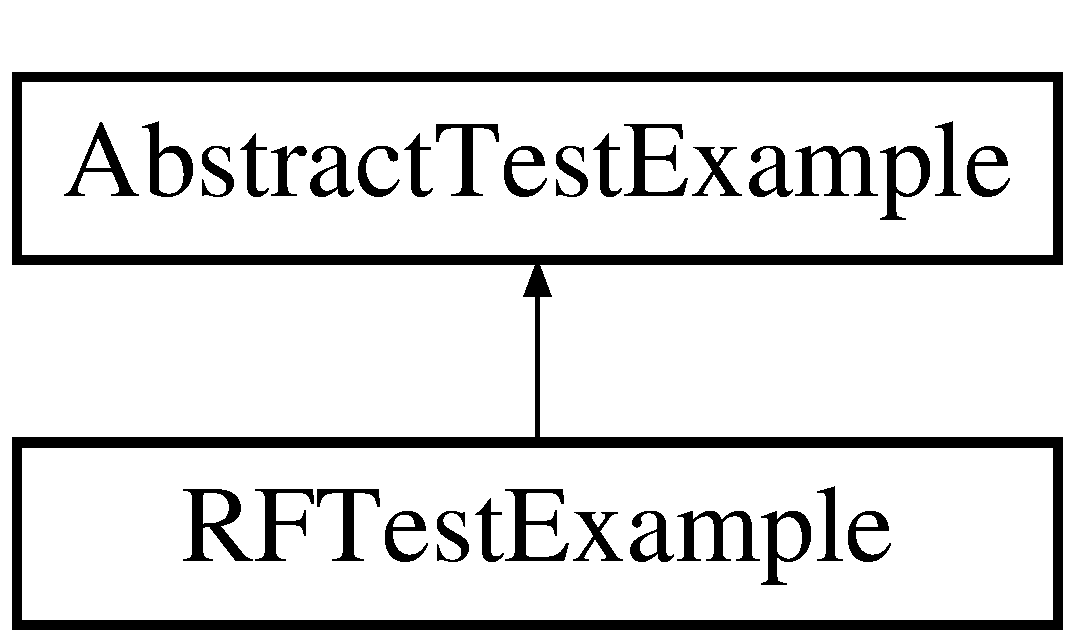
\includegraphics[height=2.000000cm]{class_r_f_test_example}
\end{center}
\end{figure}
\subsection*{Public Member Functions}
\begin{DoxyCompactItemize}
\item 
\hyperlink{class_r_f_test_example_a322a2a8b8f166fdec1c6d861c747f0dc}{R\+F\+Test\+Example} ()
\item 
\hyperlink{class_r_f_test_example_a13d41ad2a8acaaee0d19df83b813615a}{$\sim$\+R\+F\+Test\+Example} ()
\item 
virtual void \hyperlink{class_r_f_test_example_a9b935f69b49525d77dbadfa9869df17b}{Run} (int max\+Iter)
\item 
virtual void \hyperlink{class_r_f_test_example_a652c91791e5ba6ce6b89029ba0d9ac8e}{Print\+Performance} ()
\end{DoxyCompactItemize}
\subsection*{Additional Inherited Members}


\subsection{Detailed Description}
class \hyperlink{class_r_f_test_example}{R\+F\+Test\+Example} 

An test example to compare SP O\+RF, MP O\+RF, Dy\+Ba O\+RF and its offine counterpart 

\subsection{Constructor \& Destructor Documentation}
\index{R\+F\+Test\+Example@{R\+F\+Test\+Example}!R\+F\+Test\+Example@{R\+F\+Test\+Example}}
\index{R\+F\+Test\+Example@{R\+F\+Test\+Example}!R\+F\+Test\+Example@{R\+F\+Test\+Example}}
\subsubsection[{\texorpdfstring{R\+F\+Test\+Example()}{RFTestExample()}}]{\setlength{\rightskip}{0pt plus 5cm}R\+F\+Test\+Example\+::\+R\+F\+Test\+Example (
\begin{DoxyParamCaption}
{}
\end{DoxyParamCaption}
)}\hypertarget{class_r_f_test_example_a322a2a8b8f166fdec1c6d861c747f0dc}{}\label{class_r_f_test_example_a322a2a8b8f166fdec1c6d861c747f0dc}
Construction function \index{R\+F\+Test\+Example@{R\+F\+Test\+Example}!````~R\+F\+Test\+Example@{$\sim$\+R\+F\+Test\+Example}}
\index{````~R\+F\+Test\+Example@{$\sim$\+R\+F\+Test\+Example}!R\+F\+Test\+Example@{R\+F\+Test\+Example}}
\subsubsection[{\texorpdfstring{$\sim$\+R\+F\+Test\+Example()}{~RFTestExample()}}]{\setlength{\rightskip}{0pt plus 5cm}R\+F\+Test\+Example\+::$\sim$\+R\+F\+Test\+Example (
\begin{DoxyParamCaption}
{}
\end{DoxyParamCaption}
)}\hypertarget{class_r_f_test_example_a13d41ad2a8acaaee0d19df83b813615a}{}\label{class_r_f_test_example_a13d41ad2a8acaaee0d19df83b813615a}
Deconstruction function 

\subsection{Member Function Documentation}
\index{R\+F\+Test\+Example@{R\+F\+Test\+Example}!Print\+Performance@{Print\+Performance}}
\index{Print\+Performance@{Print\+Performance}!R\+F\+Test\+Example@{R\+F\+Test\+Example}}
\subsubsection[{\texorpdfstring{Print\+Performance()}{PrintPerformance()}}]{\setlength{\rightskip}{0pt plus 5cm}void R\+F\+Test\+Example\+::\+Print\+Performance (
\begin{DoxyParamCaption}
{}
\end{DoxyParamCaption}
)\hspace{0.3cm}{\ttfamily [virtual]}}\hypertarget{class_r_f_test_example_a652c91791e5ba6ce6b89029ba0d9ac8e}{}\label{class_r_f_test_example_a652c91791e5ba6ce6b89029ba0d9ac8e}
Print performance 

Reimplemented from \hyperlink{class_abstract_test_example_ab887dba326820db0a9c896ec83559e75}{Abstract\+Test\+Example}.

\index{R\+F\+Test\+Example@{R\+F\+Test\+Example}!Run@{Run}}
\index{Run@{Run}!R\+F\+Test\+Example@{R\+F\+Test\+Example}}
\subsubsection[{\texorpdfstring{Run(int max\+Iter)}{Run(int maxIter)}}]{\setlength{\rightskip}{0pt plus 5cm}void R\+F\+Test\+Example\+::\+Run (
\begin{DoxyParamCaption}
\item[{int}]{max\+Iter}
\end{DoxyParamCaption}
)\hspace{0.3cm}{\ttfamily [virtual]}}\hypertarget{class_r_f_test_example_a9b935f69b49525d77dbadfa9869df17b}{}\label{class_r_f_test_example_a9b935f69b49525d77dbadfa9869df17b}
Run the forest training and testing 
\begin{DoxyParams}[1]{Parameters}
\mbox{\tt in}  & {\em max\+Iter} & the maximal number of iteration \\
\hline
\end{DoxyParams}
get online training data 

Reimplemented from \hyperlink{class_abstract_test_example_a7ad10a9fa18201ab05fc27528a8b52e6}{Abstract\+Test\+Example}.



The documentation for this class was generated from the following files\+:\begin{DoxyCompactItemize}
\item 
/\+Users/guotaiwang/\+Documents/workspace/git\+\_\+repository/\+Dy\+Ba\+O\+R\+F/\+Test/R\+F\+Test\+Example.\+h\item 
/\+Users/guotaiwang/\+Documents/workspace/git\+\_\+repository/\+Dy\+Ba\+O\+R\+F/\+Test/R\+F\+Test\+Example.\+cpp\end{DoxyCompactItemize}

%--- End generated contents ---

% Index
\backmatter
\newpage
\phantomsection
\clearemptydoublepage
\addcontentsline{toc}{chapter}{Index}
\printindex

\end{document}
